%% This is file `sample-acmsmall-conf.tex',
%% generated with the docstrip utility.
%%
%% The original source files were:
%%
%% samples.dtx  (with options: `acmsmall-conf')
%% 
%% IMPORTANT NOTICE:
%% 
%% For the copyright see the source file.
%% 
%% Any modified versions of this file must be renamed
%% with new filenames distinct from sample-acmsmall-conf.tex.
%% 
%% For distribution of the original source see the terms
%% for copying and modification in the file samples.dtx.
%% 
%% This generated file may be distributed as long as the
%% original source files, as listed above, are part of the
%% same distribution. (The sources need not necessarily be
%% in the same archive or directory.)


%% The first command in your LaTeX source must be the \documentclass command.
\documentclass[acmsmall]{acmart}

\acmConference{}{}{}
\makeatletter
\renewcommand\@formatdoi[1]{\ignorespaces}
\makeatother
\usepackage{hyperref}
\usepackage{multicol}
\usepackage{makeidx}
\makeindex
\usepackage{float}

\hypersetup{
colorlinks=true,linkcolor=red,citecolor=green,filecolor=magenta,urlcolor=cyan
}

\usepackage{fancyhdr}
\usepackage{textgreek}
\usepackage{fixltx2e}
\usepackage[linesnumbered,ruled]{algorithm2e}
\settopmatter{printacmref=false}
\setcopyright{none}

\renewcommand\footnotetextcopyrightpermission[1]{}
\pagestyle{plain}

\settopmatter{printacmref=false} % Removes citation information below abstract
\renewcommand\footnotetextcopyrightpermission[1]{} % removes footnote with conference information in first column
\pagestyle{plain} % removes running headers


\usepackage{listings}
\usepackage{color}
\renewcommand\labelitemi{\tiny$\bullet$}

\definecolor{dkgreen}{rgb}{0,0.6,0}
\definecolor{gray}{rgb}{0.5,0.5,0.5}
\definecolor{mauve}{rgb}{0.58,0,0.82}

\lstset{frame=tb,
  language=C++,
  aboveskip=3mm,
  belowskip=3mm,
  showstringspaces=false,
  columns=flexible,
  basicstyle={\small\ttfamily},
  numbers=none,
  numberstyle=\tiny\color{gray},
  keywordstyle=\color{blue},
  commentstyle=\color{dkgreen},
  stringstyle=\color{mauve},
  breaklines=true,
  breakatwhitespace=true,
  texcl=true,
  mathescape=true,
  tabsize=3
}

%% \BibTeX command to typeset BibTeX logo in the docs
%% Rights management information.  This information is sent to you
%% when you complete the rights form.  These commands have SAMPLE
%% values in them; it is your responsibility as an author to replace
%% the commands and values with those provided to you when you
%% complete the rights form.
%% These commands are for a PROCEEDINGS abstract or paper.
%% Submission ID.
%% Use this when submitting an article to a sponsored event. You'll
%% receive a unique submission ID from the organizers
%% of the event, and this ID should be used as the parameter to this command.
%%\acmSubmissionID{123-A56-BU3}

%% The majority of ACM publications use numbered citations and
%% references.  The command \citestyle{authoryear} switches to the
%% "author year" style.
%% If you are preparing content for an event
%% sponsored by ACM SIGGRAPH, you must use the "author year" style of
%% citations and references.

\begin{document}

%% The "title" command has an optional parameter,
%% allowing the author to define a "short title" to be used in page headers.
\title{\centering Review of NG-DBSCAN: Scalable Density-Based Clustering for Arbitrary Data}

%% The "author" command and its associated commands are used to define
%% the authors and their affiliations.
%% Of note is the shared affiliation of the first two authors, and the
%% "authornote" and "authornotemark" commands
%% used to denote shared contribution to the research.
\author[1]{\centering \centerline{Group 10 - \lowercase{algo\_miners}} \newline \newline Samay Varshney - \lowercase{samay@iitg.ac.in} - 180101097 \newline Pulkit Changoiwala - \lowercase{changoiw@iitg.ac.in} - 180101093 \newline Sai Sumanth Madicherla - \lowercase{madicher@iitg.ac.in} - 180101068 \newline Komatireddy Sai Vikyath Reddy - \lowercase{komatire@iitg.ac.in} - 180101036}

%% By default, the full list of authors will be used in the page
%% headers. Often, this list is too long, and will overlap
%% other information printed in the page headers. This command allows
%% the author to define a more concise list
%% of authors' names for this purpose.

\renewcommand{\shortauthors}{Samay, Pulkit, Sumanth, Vikyath}
\renewcommand*\contentsname{\Large\textbf{Contents}}
%% The abstract is a short summary of the work to be presented in the
%% article.

\maketitle
\thispagestyle{empty}

\bibliography{sample-base.bib}

\setcounter{tocdepth}{5}
\setcounter{secnumdepth}{5}
\tableofcontents
\newpage

\section* {\centerline{Section 1: Review of the algorithm}  \newline}
\addcontentsline{toc}{section}{\large Section 1: Review of the algorithm}

\section* {Abstract}
NG-DBSCAN is an \textbf{approximated} and \textbf{distributed} density-based clustering algorithm that operates on \textbf{arbitrary data} and \textbf{any symmetric distance} measure. In this review, we provide an overview of the steps in the NG-DBSCAN algorithm along with its evaluation criteria and applications. The results are obtained through different experiments with \textbf{real and synthetic data}, proving the claims about NG-DBSCAN’s performance and scalability.
\vspace{-6pt}
\section* {Introduction}
Clustering algorithms are fundamental in data analysis, providing an unsupervised way to aid understanding and interpreting data by grouping similar objects together. \newline DBSCAN introduced the idea of density-based clustering: grouping data packed in high-density regions of the feature space. DBSCAN has \textbf{two important features}: first, it separates “core points” appearing in dense regions of the feature spaces from outliers (noise points) which are classified as not belonging to any cluster; second, it recognizes clusters having arbitrary shapes rather than being limited to ball-shaped ones. But then also, DBSCAN has many limitations which we have discussed in the next section. \newline
Even though several distributed DBSCAN implementations exist: they partition the feature space, running a single-machine DBSCAN implementation on each partition, and then "stitch" the work done on the border of each partition, all these approaches are effective only when dimensionality is low and also are not able to handle any kind of heterogeneous data.

\section* {Major Bottlenecks Solved by NG-DBSCAN}
The proposed algorithm solves the \textbf{DBSCAN scalability problem of handling large databases}, the \textbf{inconsistency of working with heterogeneous data sets}: through a modified implementation of DBSCAN which is approximated, scalable and distributed, supporting any arbitrary data and any symmetric distance measure. The modified implementation so-called NG-DBSCAN algorithm, in some of the cases even outperforms competing for DBSCAN implementations while the approximation imposes small or negligible impact on the results. \newline

\textbf{The problem with DBSCAN was that in high dimensional datasets, it partitions the feature space and then merges the spaces which lead to high computational complexity in large datasets.} Also when applied to arbitrary distance measures, it requires retrieving each point’s \textepsilon-neighborhood, for which the distance between all node pairs needs to be computed, resulting in $O(n\textsuperscript{2})$ calls to the distance function. 
NG-DBSCAN on the other hand follows a vertex centric approach in which computation is partitioned by and logically performed at the vertices of a graph, and vertices exchange messages whereby building a neighbour and \textepsilon-graph and clusters are built based on the neighbour graph content. This approach enables distribution without needing Euclidean spaces to partition.
In most of the existing DBSCAN algorithms where $d >= 6$ or n is high, it is computationally infeasible to run the algorithm either due to memory errors or large time complexity. However the algorithm mentioned in the paper named NG-DBSCAN, is \textbf{independent of the dimensionality} of the dataset and is able to run in the time \textbf{linear} to the number of data points.  


\section* {NG-DBSCAN Algorithm: An Overall Description and Flowcharts }
The NG-DBSCAN algorithm happens in two phases. Dataset is represented in the form of a graph where each node or vertex is a data point and edges represent the similarity distance measure between points. In the algorithm we are having \textepsilon, $Minpts$, $M\textsubscript{max}$, \textrho, $T\textsubscript{n}$, $T\textsubscript{r}$, k as parameters and these are tuned in accordance with the number of data points and as per most efficient computational complexity. NG notation is used for denoting Neighbour Graph here.

\begin{enumerate}
    \item \textbf{First Phase: } It is implemented through a neighbour graph which converges to k-nearest neighbour graph. It creates the \textepsilon-graph and avoids the \textepsilon-neighbourhood queries (which were creating high computational cost in DBSCAN). \newline
    The \textepsilon-neighborhood of a point p is the set of points within distance ε from p. \newline \textepsilon-neighbourhood queries for a given vertex is finding nodes that are within the \textepsilon-distance which can take upto $O(n\textsuperscript{2})$ if performed naively. \newline \textepsilon-graph nodes are data points where each node’s neighbors are a subset of its \textepsilon-neighborhood. \newline
    At each iteration, all pairs of nodes $(x,y)$ separated by 2 hops in the neighbor graph are considered and if their distance is less than \textepsilon, then this edge is added in \textepsilon-graph. To speed up the computation, nodes with at least M\textsubscript{max} neighbors are removed from the neighbour graph.
    
    \begin{figure}[!ht]
        \centering
        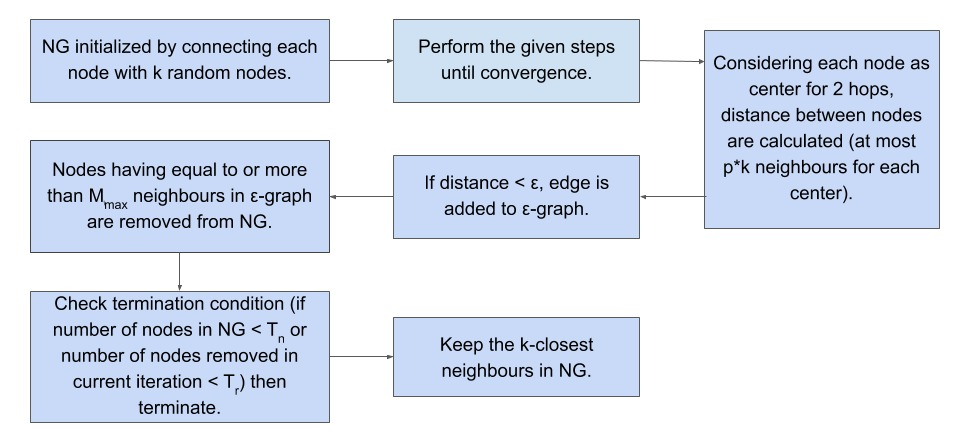
\includegraphics[width=\textwidth,height=\textheight,keepaspectratio]{Phase 1.jpeg}
        \vspace{-8mm}
        \caption{Overview of Phase 1}
        \label{fig:NG-DBSCAN Algorithm}
    \end{figure}
        
    \vspace{-2mm}
    \begin{figure}[!ht]
        \centering
        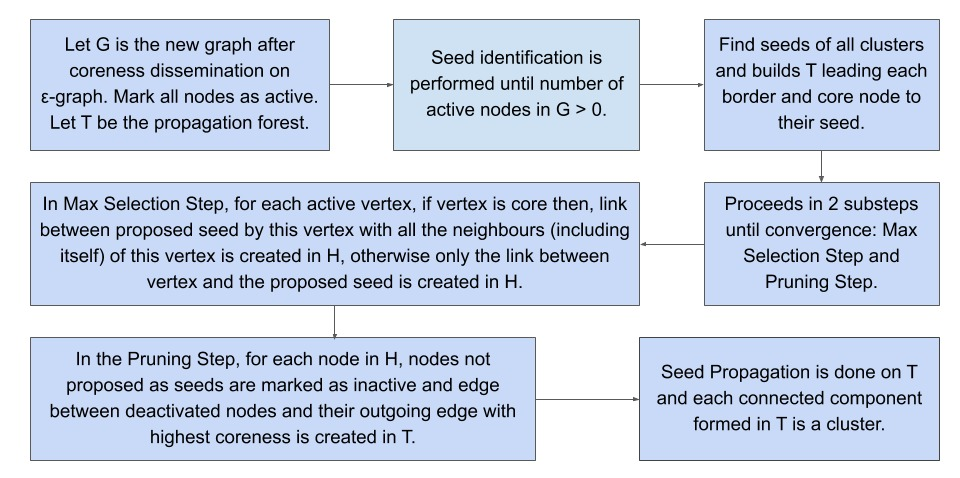
\includegraphics[width=\textwidth,height=\textheight,keepaspectratio]{Phase 2.jpeg}
        \vspace{-6mm}
        \caption{Overview of Phase 2}
        \label{fig:NG-DBSCAN Algorithm}
    \end{figure}
    
    \item \textbf{Second Phase: }
    Second phase takes \textepsilon-graph as input to build a clustering and neighbour lookups are performed instead of \textepsilon-neighbourhood queries. All nodes are given different roles in the \textepsilon-graph. \newline 
    Core nodes are those having at least $MinPts-1$ neighbours, Border nodes are those having at least 1 core node as neighbour while Noise nodes are the remaining nodes. 
    Each node coreness is then referred to as $(degree,nodeID)$. This labeling with degree is called coreness dissemination of the graph. Seed of a cluster is called a node with highest coreness. The Propagation forest is created having seed as root for each cluster and from that different clusters are created.
    
\end{enumerate}

\section* {Evaluation of the algorithm}
The evaluation of the algorithm was carried out by running it on both synthetically generated and externally used datasets and comparing the results with exact DBSCAN, by comparing its scalability against SPARK-DBSCAN and IRVINGC-DBSCAN.
\textbf{Quality metrics such as compactness, separation, recall and speed-up} are used to distinguish. \newline
Compactness measures how closely are items in each cluster. Separation measures how well items in different clusters are separated. Recall of a cluster is the fraction of the node pairs that are in the same cluster with that in a reference cluster. Speed-Up metric measures the algorithm runtime improvement when increasing the number of cores dedicated to the computation. \newline
Since computing the above metrics is computationally hard, data points are picked randomly with uniform sampling and averaging independent runs for each data point. \newline
In \textbf{2-dimensional space}, clustering quality is compared by checking time taken and recall on different datasets and scalability is measured by taking different dataset sizes and number of cores used. \newline
In \textbf{d-dimensional space}, both clustering recall and time taken are compared with the number of dimensions used in different datasets. \newline
In \textbf{textual data}, NG-DBSCAN (using both \textit{word2vec} format and 
\textit{jaro winkler’s} edit distance separately) is compared with k-means (for k-means data was converted to word2vec format), using the compactness, separation and time taken metrics. \newline
\textbf{High compactness, less separation, less time taken} was observed in most of the NG-DBSCAN cases in comparison with other DBSCAN algorithms irrespective of the data which proves that clusters are more separated, dense and efficiently computable in case of NG-DBSCAN as seen in the results of the paper.


\section* {Experiment: Code and Datasets }
We were not able to find the \textbf{Twitter} dataset and the \textbf{Spam} dataset used by the author. But we have \href{https://drive.google.com/drive/folders/1OMBY0WbDgKs0JURcQVRG8VtPgirTbuBQ?usp=sharing}{\textit{\underline{mailed}}} the author asking for the same.

We were only able to find the  \href{https://github.com/alessandrolulli/gdbscan}{\textit{\underline{implementation}}} of NG-DBSCAN in Java with Apache Spark framework.

\section* {Real World Applications}
NG-DBSCAN being a new algorithm (2016), we could not find any real-world applications that claim to use NG-DBSCAN. However, there are ample applications for it's parent algorithm "DBSCAN". And wherever DB-SCAN is used, NG-DBSCAN can be used there.
Some applications of DBSCAN (and NG-DBSCAN) are:
\begin{itemize}
\item A widespread application of DBSCAN is the geographical clustering, where the goal is to cluster geo points having geo coordinates latitude, longitude. This will be very helpful in the following cases:
\begin{itemize}
    \item To \href{https://www.oreilly.com/content/clustering-geolocated-data-using-spark-and-dbscan/}{\textit{\underline{determine}}} geographical areas that are specific and personal to each user and look at how to build location-based services by extracting users’ geographical regions from numerous geolocated events, such as check-ins in restaurants or cafes. Such a system could identify, for instance, areas that a given user typically frequents for dinner outings.
    \item When we have too much of \href{https://geoffboeing.com/2014/08/clustering-to-reduce-spatial-data-set-size/}{\textit{\underline{geo-spatial}}} data, we might need to reduce the size of a data set down to a smaller set of spatially representative points. Here we can use NG-DBSCAN to cluster them down to a smaller dataset.
\end{itemize}
\item Based on previous shows you have watched in the past, Netflix will \href{https://elutins.medium.com/dbscan-what-is-it-when-to-use-it-how-to-use-it-8bd506293818}{\textit{\underline{recommend}}} shows for you to watch next. This can be done through NG-DBSCAN clustering of people who have watched similar shows. In fact, this is a very popular use of clustering that we all might be familiar with.
\item It can be used to cluster all the emails which are similar to each other in some form which can be used as a symmetric distance measure in the algorithm for clustering.
\item It can be used to cluster all the cricketers who are similar in their batting techniques using a d-dimensional dataset where each field in d-dimension is a probability value of playing that kind of shot by the player and taking each player as a data point.  
\end{itemize}

\textbf{\textit{We have not found any ML/Data Analysis Package that includes NG-DBSCAN algorithm.}}


\section* {Conclusion}
We presented a review of NG-DBSCAN, a novel distributed algorithm for density-based clustering that produces quality clusters with arbitrary distance measures. This allows domain experts to choose the similarity function appropriate for their data, and parallelism can be addressed by designers. We showed an overview of the steps involved in the algorithm and how it is evaluated. We found out that this algorithm has lots of real-life applications and mention some of them in the review report as well.

Our next steps will be to understand the algorithm in-depth and start its implementation. Then we will propose our iterations to make it an incremental clustering algorithm.

\section* {Updates of the Dataset}
Alessandro Lulli (Author of the paper) has sent us the  \href{https://archive.ics.uci.edu/ml/datasets.php}{\textcolor{blue}{datasets}}.

\newpage

\section* {\centerline{Section 2: Related Work} \newline}
\addcontentsline{toc}{section}{\large Section 2: Related Work}

\section* {Incremental Versions}
We didn't find any incremental versions of NG-DBSCAN. But we have found some other incremental versions which are somewhat related to NG-DBCAN and DBSCAN.
\begin{enumerate}
    \item \textcolor{blue}{\textbf{\href{https://citeseerx.ist.psu.edu/viewdoc/download?doi=10.1.1.678.8143&rep=rep1&type=pdf
    }{MR-IDBSCAN: Efficient Parallel Incremental DBSCAN Algorithm using MapReduce:}}}
    It is also a scalable, density based algorithm to find clusters of arbitrary shapes, size, and as well as filter out noise like NG-DBSCAN does. It also uses the Map Reduce method which NG-DBSCAN follows. 
    \begin{itemize}
        \item \textbf{Intuition of proposed solution:} In this algorithm, new data points which intersect with old data points are determined. For each intersection point, the new dataset uses an incremental DBSCAN algorithm to determine new cluster membership. Cluster memberships of the remaining points are then updated. R*- tree data structure is used in this algorithm.
        \item \textbf{Results:} Time complexity of this algorithm is less than the original DBSCAN	algorithm and it has also dealt with fault tolerance which makes it to compete with NG-DBSCAN.
        \item \textbf{Limitations:} In this algorithm it is difficult to delete clusters incrementally from an existing set of clusters.
    \end{itemize}
    \vspace{5pt}
    \item \textcolor{blue}{\textbf{\href{https://link.springer.com/article/10.1007\%2Fs10044-019-00831-1}{BISDB$\textsubscript{x}$: Batch‑Incremental Clustering for Dynamic Datasets using SNN‑DBSCAN:}}}
    BISDB$\textsubscript{x}$ is a batch-incremental algorithm based on graph based clustering involving frequently changing dynamic datasets.
    \begin{itemize}
        \item \textbf{Intuition of proposed solution:}  Incremental version of SNNDB, a graph-based clustering technique is modified to BISDB$\textsubscript{x}$ since it was making the process extremely slow when updates are made on larger base dataset. BISDB$\textsubscript{add}$ is used while adding points while BISDB$\textsubscript{add}$ is used while deleting points dynamically. It computes K-Nearest Neighbour graph (like in case of NG-DBSCAN), shared nearest neighbours graph, core and non-core points incrementally.
        \item \textbf{Result:} Experimental observations on real world and synthetic datasets showed that BISDB$\textsubscript{x}$ are up to 4 orders of magnitude faster than the naive SNNDB algorithm and about 2 orders of magnitude faster than the pointwise incremental method.
    \end{itemize}
    \vspace{5pt}
    \item \textcolor{blue}{\textbf{\href{https://ieeexplore.ieee.org/document/8757475}{A New Incremental Semi-Supervised Graph Based Clustering: }}} \newline
     In the case of semi-supervised learning, before this paper came out, there was no incremental algorithm. This paper introduces a new incremental semi-supervised clustering which is based on a graph of k-nearest neighbor using seeds, namely IncrementalSSGC. In each incremental clustering algorithm, two processes including insertion and deletion for new data points are used for updating the current clusters.
    \begin{itemize}
        \item \textbf{Intuition of proposed solution:} Given a k-nearest neighbor graph presenting a data set X, this step uses a loop in which at each step, all edges which have weight less than a threshold $\theta$ will be removed. The value of $\theta$ is initialized by $\theta$ at first step and incremented by 1 after each step. This loop will stop when each connected component has at most one kind of seeds. The main clusters are identified by propagating label in each connected component that contains seeds. The further steps isolate the outliers.
        \item \textbf{Results:} IncrementalSSGC obtains the good results compared with the IncrementalDBSCAN. It can be explained by the fact that the IncrementalDBSCAN can not detect clusters with different densities while IncrementalSSGC does and hence is a competitor for NG-DBSCAN.
    \end{itemize}
\end{enumerate}
\vspace{1pt}

\section* {Variants}
\begin{enumerate}
    \item \textcolor{blue}{\textbf{\href{https://journalofbigdata.springeropen.com/articles/10.1186/s40537-019-0207-2}{DENCAST: Distributed Density-Based Clustering for Multi-target Regression:}}}
    
    DENCAST system, a novel distributed algorithm implemented in Apache Spark, which performs density-based clustering and exploits the identified clusters to solve both single- and multi-target regression tasks (and thus, solves complex tasks such as time series prediction). 
    \newline 
    \textit{Like NG-DBSCAN it is able to handle large-scale and high dimensional data.}
    \vspace{3pt} \newline 
    \textbf{The key features:}
    \begin{itemize}
        \item It works on the neighborhood graph. In this way, the algorithm needs only object IDs and their neighborhood relationships (instead of their initial, possibly high-dimensional, representation) and thus it requires limited space resources. We build such a neighborhood graph efficiently from high-dimensional data through the locality-sensitive hashing (LSH) method.
        \item It is implemented in the Apache Spark framework and it is fully distributed. Therefore, it does not require pre-processing or post-processing steps, usually performed on a single machine. This aspect allows our method to analyze large-scale datasets without incurring in computational bottlenecks.
        \item The identified density-based clusters can be exploited to predict the value of one or more target variables, by means of a density- and distance-based approach. The result is that the proposed method can be adopted to solve single-target and multi-target regression tasks in a distributed setting.
    \end{itemize}
    \vspace{5pt}
    \textbf{Algorithm:}
    \begin{itemize}
        \item Given the dataset consisting of n labeled objects we first apply a distributed variant of locality-sensitive hashing—LSH to identify an approximate neighborhood graph.
        \item From this point, the algorithm only uses the neighborhood graph, which can be considered an approximate representation of the objects and their distances, instead of objects represented in the original feature space.
        \item Our method for density-based clustering then maps each labeled node to a cluster by propagating cluster IDs from core objects through their neighbors. Our approach is iterative and requires a stopping criterion, based on a threshold (\textit{labelChangeRate}), aiming to avoid unnecessary iterations, which would lead to slight changes in cluster assignments. Note: p is a core object if $|N(p)| \geq MinPts$
    \end{itemize}
    \vspace{8pt}
    
    \item \textcolor{blue}{\textbf{\href{https://link.springer.com/article/10.1007/s11704-013-3158-3}{MR-DBSCAN: A Scalable MapReduce Based DBSCAN Algorithm:}}}
    \newline
    MR-DBSCAN consists of three stages: data partitioning, local clustering, and global merging. The first stage divides the whole dataset into smaller partitions according to spatial proximity. In the second stage, each partition is clustered independently. Then the partial clustering results are aggregated in the last stage to generate the global clusters.
    \newline
    Let S\textsubscript{u} denote the minimum bounding rectangle (MBR) of all the input points in \textbf{\textit{DB}}. During data partitioning, we divide S\textsubscript{u} into non-overlap sub-rectangles. All the input points in \textbf{\textit{DB}} that fall into or close to a rectangle form a partition. The local clustering stage performs sequential DBSCAN for each data partition separately and save the local clusters as intermediate results. \newline
    Sequential merging of local clusters becomes inefficient when dealing with very large datasets. To address this problem, a parallel algorithm is proposed to ensure the scalability of this stage.
 
    \vspace{8pt}
    
    \item \textcolor{blue}{\textbf{\href{https://arxiv.org/pdf/2009.04552.pdf}{KNN-DBSCAN: DBSCAN in High Dimensions:}}}
    \newline
    To enable density clustering of high-dimensional datasets we propose a DBSCAN algorithm that uses an approximate k-Nearest-Neighbor graph (k-NNG). For the exact k-NNG, an edge E\textsubscript{ij} between vertices i,j exists if and only if p\textsubscript{j} is in the k-nearest neighbor list of i. 
    \newline
    Notice that k-NNG is a directed graph—in contrast to $\epsilon$-NNG. The main reason k-NNG is used is that we can probably control the work and memory complexity. That is, memory requirements for k-NNG always remain $O(n*k)$, whereas for $\epsilon$-NNG can explode to $O(n^{2})$.
    \newline
    Instead of running out of memory or creating severe load imbalance as is often the case with $\epsilon$-NNG, k-NNG only suffers from a loss in accuracy. But convenient as k-NNG is, DBSCAN requires a symmetric $\epsilon$-NNG. To circumvent this, kNN-DBSCAN is introduced that uses the k-NNG. 
 
\end{enumerate}

\newpage
\section* {\centerline{Section 3: Code Architecture} \newline}
\addcontentsline{toc}{section}{\large Section 3: Code Architecture}

\section* {Class Definitions and Data Structures}
In terms of data structures, \textbf{graphs}, \textbf{lists} and \textbf{priority queues} are used. Some of the classes used are listed below.
\begin{lstlisting}
class Node {
    id              -   represents node ID
    degree          -   represents number of edges connected to this node
    coreness        -   represents (id, type) of node
    coordinates     -   represents the data point from our dataset
    type            - 	represent whether Node is core, border or noise
    Node(id){       - 	constructor to initialize Node
        this.id = id
        this.type = none
    }
}
class Graph { 
    int N 					              -	Total number of nodes
    set<Node> active 			        - 	List of active nodes
    vector<Node,int> edges[N] 	     -	Adjacency List
    Graph(int total_nodes) {
    	this.active = {$u  \forall u \in N$}                // make all nodes as active
    	this.N = total_nodes
    }
    void remove_node(Node ID)       // removes node from graph
    void add_node(Node ID)          // adds node in graph
    void remove_edge(x, y, w)       // removes edge between node x and y with weight w
    void remove_edge(x, y)          // removes edge between node x and y
    void add_edge(x, y)          // adds edge between node x and y
    void add_edge(x, y, w)          // adds edge between node x and y with weight w
    vector<Node> neighbours(x)      // returns all neighbours of node x
}
class Parameters {
	$k$		     -	represents degree of each node in neighbour graph
	$Minpts$           -   each core node is having degree at least $Minpts-1$
    T$\textsubscript{n}$         -   limits number of nodes in NG for termination
    T$\textsubscript{r}$	        -   limits number of removed nodes in current iteration in NG
    M$\textsubscript{max}$         -	used to reduce NG in phase-1 to reduce computation
    $\rho$          -   limits nodes for which 2 hop distance is calculated in NG
    $iter$          -	used to achieve convergence condition
	Parameters() {
	    // initialise all with default values unless explicit values are given
    }
}
\end{lstlisting}

\section* {Procedures}
Here are the procedures which will be used in the implementation of NG-DBSCAN algorithm. \newline
In Phase 1, the main function to be called is \textit{$\epsilon$-graph\_construction} which will use other procedures listed below.
\subsection* {Phase 1:}
\begin{lstlisting}

// creating $\epsilon$-graph
Graph $\epsilon$-graph_construction(int total_points){
	Graph $\epsilon G$(total_points), NG(total_points)
	Random_Initialisation(NG)       // initialising each node with k random edges
	delta = 0                       // number of nodes removed in current iteration
	while(i < iter and not Terminate(NG, delta)){
	    Reverse_Map(u, NG)  $\forall u \in NG$
	    Check_Neighborhood(u, NG, $\epsilon G$)  $\forall u \in NG$
	    Reduce_NG(u, NG, $\epsilon G$)  $\forall u \in NG$
        i++
    }
    return $\epsilon G$
}
void Reverse_Map(Node n, Graph G) {
    // Making the graph undirected
	for each u in G.neighbours(G) {
		w = distance(v, u)
		G.add_edge(u, v, w)
	}
}
// checking neighbour graph and updating $\epsilon$ graph
void Check_Neighborhood(Node n, Graph NG, Graph $\epsilon G$) {
    N = Random selection of at most $\rho k$ nodes from NG.neighbours(n) 
	for each vertex v in N {
		for each vertex u in N$\setminus${v} {
			w = distance(u, v)
			NG.add_edge(u, v, w)
			if(w <= $\epsilon$)
		        $\epsilon G$.add_edge(u, v, w)
        }
    }
}
// checking termination condition
bool Terminate(Graph NG, int delta){
	if(|NG.nodes| < $T\textsubscript{n}$ and delta < $T\textsubscript{r}$){
		return 1
	} 
	else {
		return 0
	}
}
// reducing neighbour graph
void Reduce_NG(Node u, Graph NG, Graph $\epsilon G$){
	if(|$\epsilon G$.neighbours(u)| >= M$\textsubscript{max}$){
	    NG.remove_node(u)
	    delta = delta + 1
	}
	vector<Node> l = NG.neighbours(u) 
	remove from l the k edges with smallest weights using priority queue
    for(u, v, w) in l {
        NG.delete_edge(u, v, w)
	}
}
\end{lstlisting}

\subsection* {Phase 2:}
In Phase 2, main function to be called is \textit{Discovering\_Dense\_Regions} which will further call other procedures listed below.

\begin{lstlisting}
// finding all the clusters
Graph Discovering_Dense_Regions(Graph $\epsilon$-NN, int total_nodes){
	// Make all nodes active
	Graph T(total_nodes)
	G = Coreness_Dissemination($\epsilon$-NN, total_nodes)
	while G has active nodes { 
		Graph H(total_nodes) 
		// Seed identification process
		Max_Selection_Step(n, G, H) $\forall n \in G$
		Pruning_Step(n, T, H, G) $\forall n \in H$
	}
	return Seed_Propagation(T)
}
// return maximum core node from the list
int Max_Core_Node(vector<Node> list){
	// returns node from list having maximum coreness value
}
void Max_Selection_Step(Node u, Graph G, Graph H){
	vector<Node> NNg = G.neighbours(u)
	int u$\textsubscript{max}$ = Max_Core_Node(NNg $\cup$ {u})
	if(u.type != core){
	    H.add_edge(u, u$\textsubscript{max}$)
    } 
    else {
    	for each node v in NNg 
            H.add_edge(v, u$\textsubscript{max}$)
    }
    H.add_edge(u$\textsubscript{max}$, u$\textsubscript{max}$)
}
// in pruning, nodes not proposed as seeds(those with no incoming edges) are deactivated
void Pruning_Step(Node u, Propagation_Tree T, Graph H, Graph G){
	vector<Node> NNh = H.neighbours(u)
	int u$\textsubscript{max}$ = Max_Core_Node(NNh)
	if(u.type != core){
	    G.remove_node(u)
	    T.add_edge(u$\textsubscript{max}$,u)
    } 
    else {
    	for each node v in (NNh \ {u$\textsubscript{max}$}){
    	    G.add_edge(v, u$\textsubscript{max}$)
    	    G.add_edge(u$\textsubscript{max}$, v)
        }
        if u not present in NNh {
    	    G.remove_node(u)
    	    T.add_edge(u$\textsubscript{max}$,u)
        }
    }
}
// convert graph to identify all nodes and return it
Graph Coreness_Dissemination(Graph $\epsilon$-NN, int total_nodes) {
	// Here we identify the core, boundary and noise points of the input ε-graph.
	Graph G(total_nodes)
	G = $\epsilon$-NN
    for each node v in G.nodes {
		if(|G.neighbours(v)| >= $Minpts-1$)
			v.type = core   // Make it a core node
	}
    for each node v in G.nodes \ {core nodes} {
		if there is at least one core node in G.neighbours(v)
			v.type = border // Make it a border node
	}
    for each node v in G.nodes \ {core nodes} \ {border nodes} {
		v.type = noise      // Mark them as noise points
		G.remove_node(v)    // We need to remove all the noise points from G
	}
    return G;
}
Graph Seed_Propagation(Graph T) {
    a = List of all seeds 
    for all nodes v in a {
    	Perform Depth First Search on graph T with v as input. 
    	// Here we will get all the nodes belonging to the cluster of v
    }
    // The final output will be a list of lists where each list corresponds to a separate cluster
}
\end{lstlisting}
In the Seed\_Propagation function, we use the already known \textbf{DFS (Depth First Search)} algorithm to find all the reachable nodes from a given node.
The list of all seeds will be obtained at the end of Seed\_Identification step. At the end of the last Pruning Step, the H graph contains only seeds and all the seeds would be present in the H graph.
Therefore DFS can be performed with all the seeds. The number of seeds will be the number of clusters formed. \newline

We will require 3 Graphs for Phase 2: Graph G, H and T.
Here G and H don’t have any precise name as their structure keeps changing with time. The aim of G and H is to ultimately obtain the “T” graph. The “T” graph is the Propagation Forest. \newline
The “T” graph contains several trees where the nodes of each tree are considered to form one cluster and the root of the tree will be the seed of the cluster(core node with maximum coreness which can be thought of as representing the whole cluster). \newline
After obtaining the “T” Graph, we call the Seed\_Propagation function which will recover the clusters from the “T” Graph.



\newpage
\section* {\centerline{Section 4: Coding Of Static Algorithm, Part 1} \newline}
\addcontentsline{toc}{section}{\large Section 4: Coding Of Static Algorithm, Part 1}

\section* {Coding Phase}
Since we didn't find any existing implementation of the algorithm in C++ or any preferable language, the \textbf{major work which we have done is writing the complete algorithm code in C++.}  \newline
We also tried much to reach to the authors regarding the existing implementation of C++ code and other resources but we didn't receive any c++ implementation from their side. They have given Scala implementation of the algorithm, but we thought of coding on our own, as understanding Scala would have taken more time.

\textcolor{blue}{\href{https://drive.google.com/drive/folders/1qXk9RKSXG47IISBB_Ycw-k5h4aKPDc4_?usp=sharing}{Mails}} and \textcolor{blue}{\href{https://github.com/alessandrolulli/gdbscan}{Scala Code}}


\section* {Code Files}
Currently our code clusters the data set consisting of 2-dimensional points. We have generated some random data points using python in a file named points.txt and these points are taken as input points for the C++ algorithm code. Then using our C++ algorithm, we have created a lists of list of points inside C++ program where each list will be a seperate cluster. Then we have written these points in a cluster.txt file and then this cluster.txt file will be used by a clusters$\_$generator.py file which will create clusters in 2-dimension. We have considered for now the distance between 2 points as the euclidean distance between them. \newline

\textcolor{blue}{\href{https://drive.google.com/drive/folders/1wbLkR-BecbqGR8qKKggDeKDug44drfDI?usp=sharing}{Code}} 

Here is the explanation of the conventions of the files used while writing the code:
\begin{itemize}
    \item \textbf{classes.h - } contains all the used classes in the algorithm.
    \item \textbf{phase1.cpp - } contains the phase-1 code which will be used to create $\epsilon$-graph.
    \item \textbf{phase2.cpp - } used to create the propagation tree and list of clusters.
    \item \textbf{epsilon$\_$graph.txt - } represents the epsilon graph used in the algorithm.
    \item \textbf{propagation$\_$tree.txt - } represents the propagation tree generated by the algorithm.
    \item \textbf{points.txt - } contains the randomly generated points used as input in phase2.cpp.
    \item \textbf{clusters.txt - } contains the lists of list of clusters.
    \item \textbf{galaxy$\_$type$\_$dataset.py - } contains the python code to generate the random points.
    \item \textbf{clusters$\_$generator.py - } plots the clusters in 2-dimension in different colours using clusters.txt.
\end{itemize}
First, galaxy$\_$type$\_$dataset.py is executed which will take as input \textbf{number of points}. Then phase2.cpp will execute. Then clusters$\_$generator.py will generate clusters (different colours denoting different clusters generated by our algorithm) using matplotlib library. \newline
Here are some instructions to run the codes:
\begin{itemize}
    \item \textbf{galaxy$\_$type$\_$dataset.py - } \textit{python3 galaxy$\_$type$\_$dataset.py}
    \item \textbf{phase2.cpp - }
        \begin{itemize}
            \item Compilation:  \textit{g++ phase2.cpp}
            \item Execution:  \textit{./a.out}
        \end{itemize}
    \item \textbf{clusters$\_$generator.py - } \textit{python3 clusters$\_$generator.py}
\end{itemize}

\section* {Evaluation}
Currently we have evaluated it for 2-dimensional points with galaxy type dataset only. Currently our algorithm is able to run for the number of points upto 100000. It can also run above these number of points but since the C++ compiler is not able to support much memory, hence we are getting segmentation fault (memory limit exceeded) for $number of points > 100000$. Also for higher K, it is not supporting.
Plot Graphs For Our Input Dataset: 
\textcolor{blue}{\href{https://drive.google.com/drive/folders/1vxzHzqo1U0bi-ouwb869wfAPm7_88NTk?usp=sharing}{Plot}}

In \textit{clusters$\_$generator.py}, we have the code generated for one of the following clusters.

\section* {Cluster Plots}
\begin{figure*}[!h]
        \centering
        \includegraphics[width= 0.7\textwidth, height=0.7\textheight, keepaspectratio]{2 Clusters.jpeg} 
        \caption{Clusters With K = 10}
        
\end{figure*}

We tried changing the parameters used in the code to see the effect of change on the cluster quality. 

For the following points distributions, we found the cluster for k = 3 and k = 10 respectively. After analysing the plots, we found that with k = 10 we are getting better results.
\textit{Left Image is with Clusters k = 3 and Right Image is with Clusters k = 10.}
Here $T\textsubscript{n}$, $T\textsubscript{r}$ are very small.
\begin{figure*} [!h]
        \centering
        \includegraphics[width=.48\textwidth]{3 Clusters_0.jpeg} 
        \includegraphics[width=.48\textwidth]{3 Clusters_1.jpeg}
        \caption{Clusters With K = 3}
        \caption{Clusters With K = 10}
        
\end{figure*}

\newpage
For the following points distributions, we changed $T\textsubscript{n}$, $T\textsubscript{r}$ majorly.

\begin{figure*} [!h]
        \includegraphics[width=.48\textwidth]{fig6.jpeg}
        \includegraphics[width=.48\textwidth]{fig7.jpeg}
        \caption{Clusters With $M\textsubscript{max}$ = 20, $epsilon$ = 10, $T\textsubscript{n}$ = 0.01*n, $T\textsubscript{r}$ = 0.001*n} 
        \caption{Clusters With $M\textsubscript{max}$ = 10, $epsilon$ = 12, $T\textsubscript{n}$ = 0.001*n, $T\textsubscript{r}$ = 0.0001*n}
\end{figure*}

\section* {Further Work}
For the next week we are planning to generalise the distance computations. We will use different evaluation metrics which we have mentioned earlier in our report to test our algorithm and compare them with mainly DBSCAN (and different variants of it if possible). We also haven't tuned our parameters properly till now so we will also work upon this. We have not completed the testing of the algorithm on the datasets used by the author in the publication and will work upon that also. We will also try to create it as arbitrary symmetric as much as possible.

Apart from these we will think which part of the code needs to be modified to convert it into an incremental algorithm.


\newpage
\section* {\centerline{Section 5: Coding Of Static Algorithm, Part 2} \newline}
\addcontentsline{toc}{section}{\large Section 5: Coding Of Static Algorithm, Part 2}
Here is the link to the github repository of the NG-DBSCAN algorithm: \textcolor{blue}{\href{https://github.com/Data-Mining-CS568/NG-DBSCAN}{Link}}.

\section*{Code Walk through}

Our algorithm generates density based clustering for given data set using NG-DBSCAN algorithm. 

In phase2.cpp, the algorithm is running from the main function. First we asked whether user wants to change the default parameters or not. \newline

\includegraphics[width=.60\textwidth]{running_ngDbscan.jpeg}
\newline \newline
\textbf{About points.txt: }
We are assuming that all the input data (textual, dimensional or randomly generated) will be present in points.txt. First line will contain dataset type (text or non-text), total number of points and dimension of the data (we assumed 0 dimension for textual data for simplicity). In rest of the lines, each line will represent a point.\newline
Then we read all the points from points.txt depending upon whether our dataset is textual or not and call epsilon\_graph\_construction function which will return $\epsilon$-graph using phase1.cpp and we will use this graph as parameter to Dense\_Discovery\_Regions function and it will return propagation forest (T).
\newline 
In Seed\_Propagation function, clusters.txt and numbered\_clusters.txt are generated. \newline
\textbf{About clusters.txt: } All the clusters generated will be present in clusters.txt. First line will contain number of clusters generated and dimension of dataset. Then in further lines, for each cluster, number of clusters present in current cluster is in seperate line followed by each point/sentence of that cluster in seperate lines.  \newline
\textbf{About numbered\_clusters.txt: } All the clusters with the number/index of each point will be present in numbered\_clusters.txt. 
\newline
\textbf{About classes.h: } We defined different important variables for our convinience here. dataset\_type variable will denote the type of dataset taken (textual or non-textual). In case of non-textual dataset, coordinates vector will store all the points. coordinates[i] will denote ith point of our dataset. In case of textual dataset, sentences will store all the sentences. sentences[i] will denote ith point of our dataset. node\_from\_id map will store each index of point to the actual point of Node datatype which contains all information about that point.

\section*{Computations of the algorithm}
We used matplotlib in generate\_clusters.py to generate the clusters for 2 and 3 dimensional datasets.

Apart from this, we used different metrics of seperation, compactness and recall to calculate how accurate our algorithm is working. metrics\_main.cpp will calculate the seperation, compactness and recall using clusters.txt for the dataset of points present in points.txt. 
\newline \newline
For the textual data, we are using jaro winkler's algorithm (as used by the author of the paper) to calculate distance between two points. jaro\_winkler\_distance.cpp contains the code to calculate distance between 2 textual points and it is used in phase2.cpp. \newline
We have also tried to compare our algorithm with DBSCAN algorithm using the above metrics. We ran the same dataset on both the NG-DBSCAN and DBSCAN and compared their metrics.

\section*{Toy Dataset}
We have taken 15 two-dimensional points as an input of the toy dataset. These points are present in file named toy\_dataset.txt. \newline
The points of toy dataset are listed below. First line represents that it is non textual data, has 15 points and is of 2 dimension. We took 2-dimensional for our simplicity in explaining. \newline
The 1st column represents x-coordinate while 2nd column represents y-coordinate of the points. ith row represents ith point. \newline
\begin{figure*} [!h]
    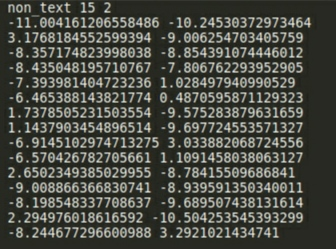
\includegraphics[width=.55\textwidth]{toy_dataset_points.jpeg}
    \caption{Toy Dataset Points} 
\end{figure*}
In phase2.cpp, we entered the following values of parameters for toy dataset. \newline
\begin{figure*} [!h]
    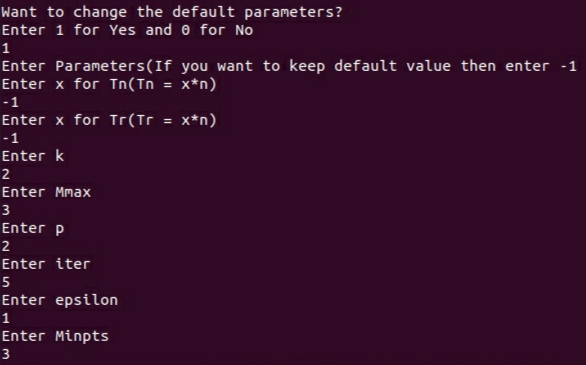
\includegraphics[width=.55\textwidth]{toy_dataset_parameters.jpeg}
    \caption{Toy Dataset Parameters} 
\end{figure*}
The red edges between (i,j) indicates the edge between the ith and jth point in the epsilon graph. Each point in the epsilon graph is connected to atleast $M\textsubscript{max}$ more points in their neighbour (as seen in the figure) which are within $\epsilon$ distance here. \newline
\begin{figure*} [!h]
    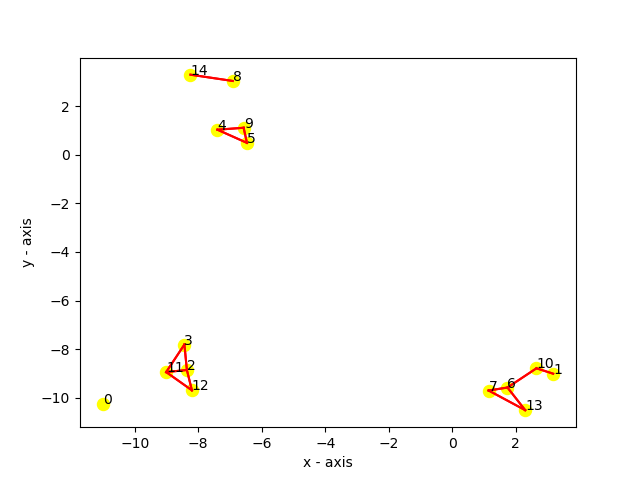
\includegraphics[width=.60\textwidth]{toy_dataset_epsilonG.png}
    \caption{Toy Dataset Epsilon Graph} 
\end{figure*}
The propagation tree is having 2nd, 4th, 6th points as seeds of different clusters and hence 3 clusters are formed. \newline
We found that the points 0th, 8th and 14th are noise since no core node is present in their neighbour within $\epsilon$ distance, while 1st point is border since only one core node (10th) is present in it's neighbour, while others are core points.
\begin{figure*} [!h]
    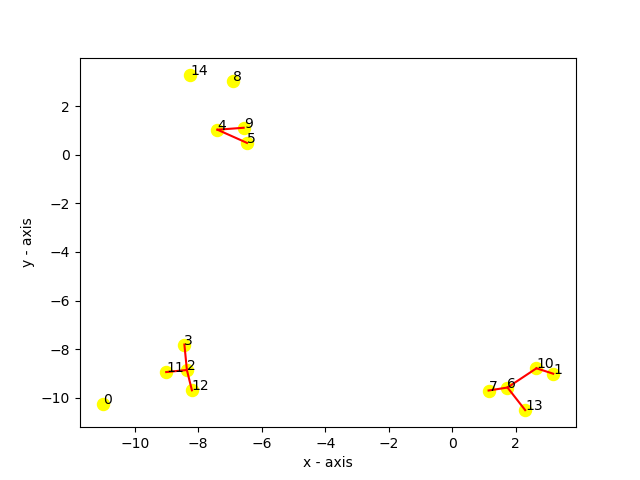
\includegraphics[width=.60\textwidth]{toy_dataset_prop_tree.png}
    \caption{Toy Dataset Propagation Tree} 
\end{figure*}
\begin{figure*} [!h]
    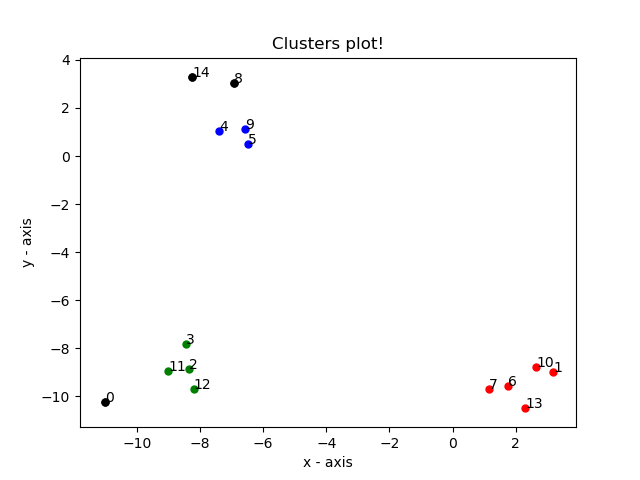
\includegraphics[width=.60\textwidth]{toy_dataset_clusters.png}
    \caption{Toy Dataset Clusters Identification} 
\end{figure*}
In the toy dataset identification of clusters, black points refer to the noise points while green points corresponds to 1st cluster and blue corresponds to 2nd cluster and red corresponds to 3rd cluster.

\section*{Text Data Compatibility}
We have added text data compatibility in the algorithm. For this we are using Jaro-Winkler's Distance Algorithm.

Using Jaro-Winkler's Distance between two strings, we define their distance to generate their epsilon graph. Then with the epsilon graph we generate the clusters for the data set in similar fashion as with Euclidean distance measure.

In dataset\_generator.py we ask user, the type of data to generate. In the points.txt(our dataset file) we are adding "text" or "non\_text" to differentiate between two types of data set.
We used the fact in comparison of strings that, the lower the Jaro–Winkler distance for two strings is, the more similar the strings are.

\newpage 
\section* {\centerline{Section 5: Proposed Incremental Algorithm, Iteration 1} \newline}
\addcontentsline{toc}{section}{\large Section 5: Proposed Incremental Algorithm, Iteration 1}

\section*{Introduction}
Many real-world applications such as search engines and recommender
systems are expected to work over dynamic datasets. Such datasets undergo
frequent changes where some points are added and some points are deleted. A
naive method to get exact clustering over the changed dataset is to run the
clustering algorithm again. Most of the computation in reclustering is going to be redudant. This problem becomes more severe with increase in frequency of updates to dynamic datasets. 

To overcome this problem, we are proposing an incremental version of NG-DBSCAN algorithm, for which we have proposed static version earlier, the incremental version will process frequent updates to dynamic datasets efficiently by avoiding redundant computation. Our incremental NG-DBSCAN will yield
significant speed-up factors over NG-DBSCAN even for large numbers of daily updates.

\section*{Description and working of the incremental version}
Our incremental version will happen in 2-phases like in case of static NG-DBSCAN. Sets of updates are processed one at a time without considering the relationships between the single updates.

\begin{enumerate}
    \item \textbf{Identification of nodes during addition and deletion:} In the static version of NG-DBSCAN, we identify each node as core and non-core (border and noise points). Here also we will maintain each node coreness with it's degree. To do this, we will maintain a set of points I, which will contain all the points for which we need to gather some information to classify them as core or non-core. This set will change during insertion and deletion of points. Here also we are using the convention that the points having atleast \textit{Minpts} neighbours are core nodes. 
    \begin{itemize}
        \item \textbf{Addition of a point:} Denote the point to be added as 'p'. While adding 'p' to our existing dataset, some of the existing points from dataset can change from non-core to core. So we insert 'p' to the set I. Those points which are having their degree as \textit{Minpts-1} are also added to the set since there is a chance that they become core due to the addition of 'p'. \\
        Our incremental algorithm analyses only the region affected by the insertion of point. The region affected by addition will be $\epsilon$-neighbourhood of point p and all points density reachable from any point in N\textsubscript{$\epsilon$}(p). Here N\textsubscript{$\epsilon$}(p) denotes the $\epsilon$-neighbourhood of p. \\ \\ \textbf{Mathematically:} \textit{Affected}\textsubscript{$D$}(p) = N\textsubscript{$\epsilon$}(p) $\cup$ $\{$ q | $\exists$ o $\in$ N\textsubscript{$\epsilon$}(p) $\land$ q >\textsubscript{D$\cap$p}o $\}$ \\ Here, x >\textsubscript{D} y, denotes y is density reachable from x w.r.t data set D. \\ \\  
        We generate a set \textit{UpdSeed\textsubscript{Ins}} which contains all core nodes in the epsilon neighbourhood of newly identified core nodes. (As adding point \textit{p} can make some points core nodes).\\ \\ \textbf{Mathematically:} \textit{UpdSeed\textsubscript{Ins}} = \{q | q is a core object in D $\cup$ \{p\}, $\exists$ q’: q’ is core object in D $\cup$ \{p\} but not in D and q $\in$ N\textsubscript{$\epsilon$}(q')\} \\ \\
        \textbf{Efficient computation of N\textsubscript{$\epsilon$}(p)}:
        \begin{itemize}
            \item For all the points 'u' in I, and for each cluster 'c' in the propagation tree, we will randomly assign k edges from 'u' with 'c'. 
            \item Let all those vertices form a set S. Then for some constant number of iterations and while 'u' is non-core (degree of 'u' < \textit{Minpts}), for each vertex 'v' in S, we will check distance between 'u' and 'v'. 
            \item If distance is <= $\epsilon$, edge is created between 'u' and 'v' and degree of 'u' and 'v' both are increased. Then we insert all the neighbours of 'v' in S. 
    
            \item Since we only require some number of points \textit{(Minpts)} within $\epsilon$ distance from 'u' to classify it as core, if this vertex is actually a core vertex after addition of it to the data set, then after some number of iterations it will eventually find some vertices of that cluster in the above process that are within $\epsilon$ distance from it. \\
        \end{itemize} 
     
        \textbf{Efficient computation of \textit{UpdSeed\textsubscript{Ins}}}:
        \begin{itemize}
            \item While running the main algorithm we store the count of number of neighbours of every point.
            \item Let denote newly identified core node as q'.
            
            \item Then, q' will be change into core node if q' $\in$ N\textsubscript{$\epsilon$}(p) and initial number of neighbours of  q' is \textit{MinPts - 1}.
            
            \item Now we need to discover neighbourhood of q' for all q which are core nodes.
            
            \item As N\textsubscript{$\epsilon$}(p) is already present in the memory, we search for neighbour of q' first there, then only we query neighbourhood of q’ and perform an additional region query only if there are more objects in the neighborhood of q’ than already contained in N\textsubscript{$\epsilon$}(p). \\ 
        \end{itemize}
        
        \begin{figure}[!h]
            \centering
            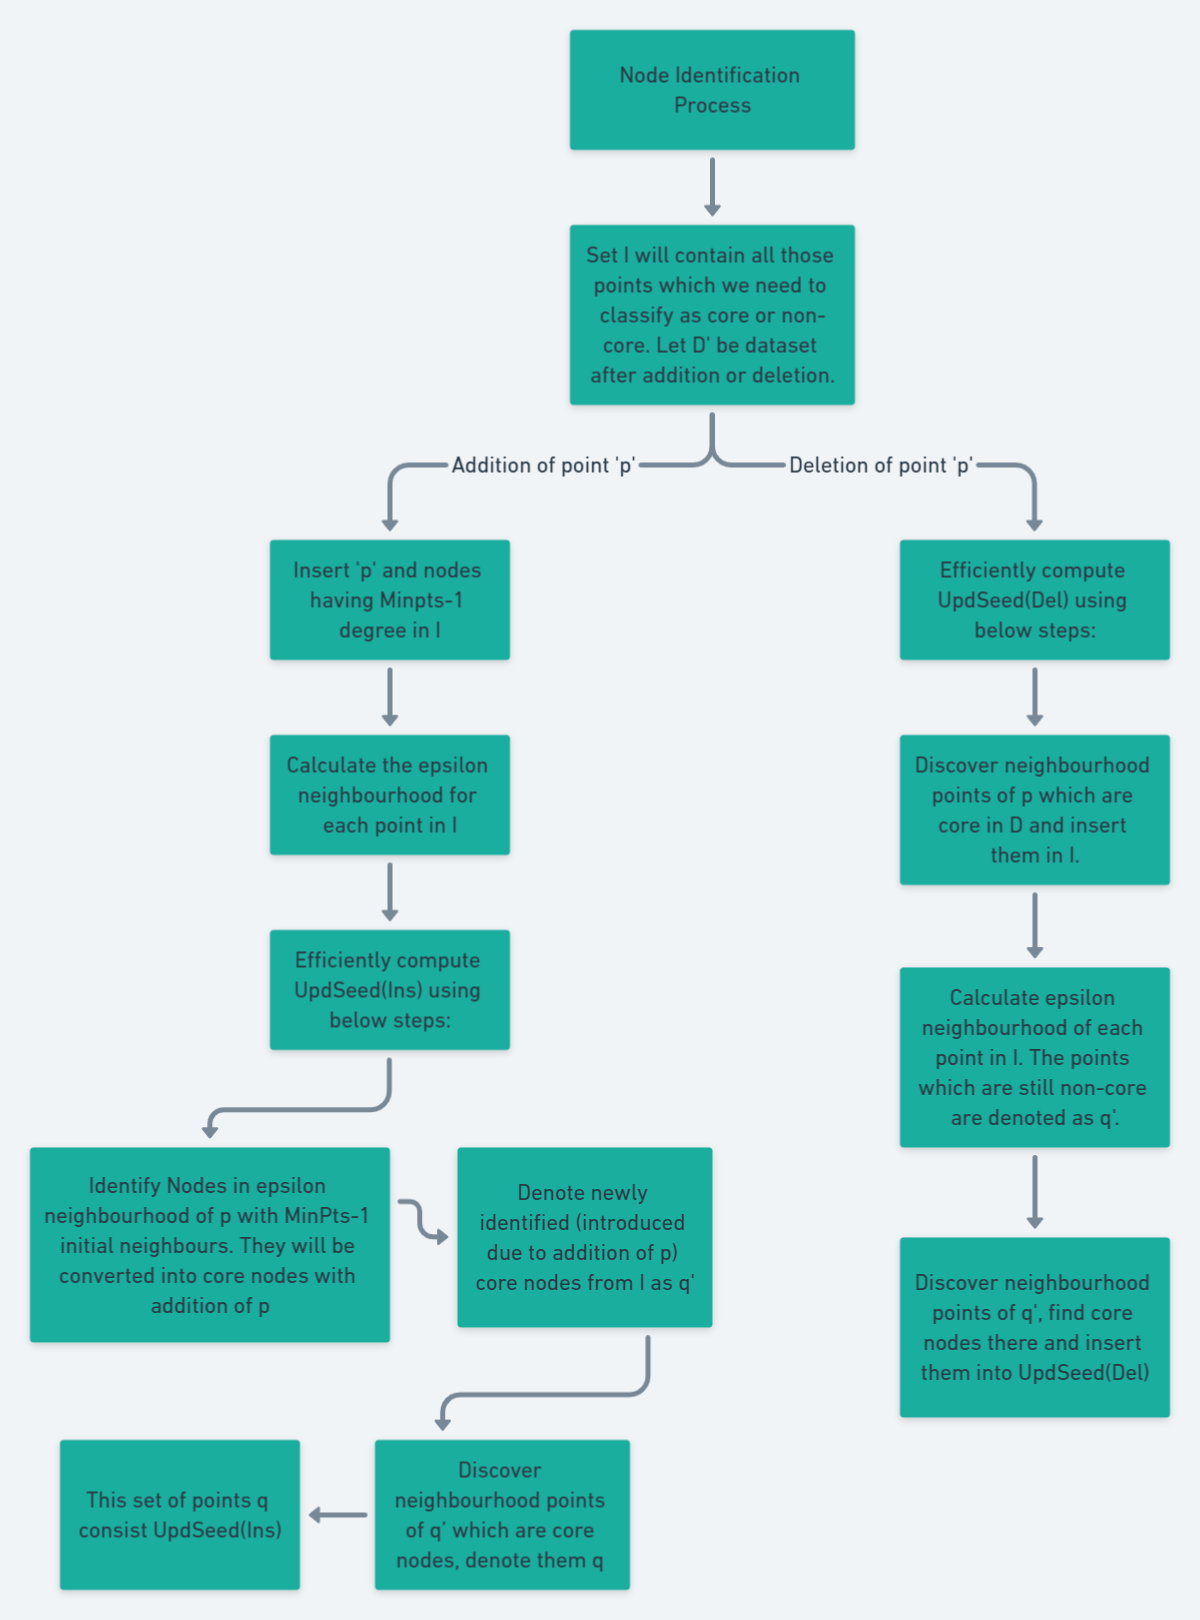
\includegraphics[width = \textwidth]{UpdSeed Construction Flow chart.png}
            \caption{UpdSeed Construction}
            \label{fig:my_label}
        \end{figure}
        
% **************** Deletion Of Point ****************
        \item \textbf{Deletion of a point:} Denote the point to be deleted as 'p'. While deleting 'p' from our existing dataset, some of the points can have their degree changed to \textit{Minpts-1} due to their loss of connection with 'p'. So we will store all those core points in I which were in the $\epsilon$-neighbourhood of 'p' since they can become non-core and we could gather some more information regarding these points whether they can become core again or not by checking their neighbourhood. \newline
        Let \textit{Affected}\textsubscript{$D$}(p) is the region affected by the deletion of point. \\ \\
        We generate a set \textit{UpdSeed\textsubscript{Del}} which contains all core node in $\epsilon$-neighbourhood of newly identified non-core nodes. (As deleting point \textit{p} can make some points non-core from core).\\ \\ \textbf{Mathematically:} \textit{UpdSeed\textsubscript{Del}} = \{q | q is a core object in D\textbackslash \{p\}, $\exists$ q’: q’ is core object in D but not in D\textbackslash \{p\} and q $\in$ N\textsubscript{$\epsilon$}(q')\} \\ \\
        \textbf{Efficient computation of N\textsubscript{$\epsilon$}(p)}:
        We already have $\epsilon$-neighbourhood of p as p was present in the data set before deletion.\\ \\
        \textbf{Efficient computation of \textit{UpdSeed\textsubscript{Del}}}:
        \begin{itemize}
            \item While running the main algorithm we store the count of number of neighbours of every point.
            \item Let denote core node in original clustering as q'.
            \item Then, q' will be change into non core node if q' $\in$ N\textsubscript{$\epsilon$}(p) and initial number of neighbours of  q' is \textit{MinPts}.
            \item Now we need to discover neighbourhood of q' for all q which are core nodes.
            \item As N\textsubscript{$\epsilon$}(p) is already present in the memory, we search for neighbour of q' first there, then only we query neighbourhood of q’ and perform an additional region query only if there are more objects in the neighborhood of q’ than already contained in N\textsubscript{$\epsilon$}(p). \\ \\
        \end{itemize}
        
        
    \end{itemize}

    \item \textbf{Cluster membership assignment: } Here we perform the merging, seperation of clusters, formation of new clusters due to addition and deletion of points. \newline 
    
    \begin{itemize}
        \item \textbf{Addition of a point: }
        When inserting a new object p, new density-connections may be established, but none are removed. In this case, it is sufficient to restrict the application of the clustering procedure
        to the set {UpdSeed\textsubscript{Ins}}. If we have to change cluster membership for an object from C to D we perform the same change of cluster membership for all other objects in C. Changing cluster membership of these objects does not involve the application of the clustering algorithm but can be handled by simply storing the information about which clusters have been merged.
        When inserting an object p into the database D, we can
        distinguish the following cases:
        \\ 

        \begin{enumerate}
            \item \textbf{Noise: }
            {UpdSeed\textsubscript{Ins}} is empty, i.e. there are no “new” core objects after insertion of p. Then, p is a noise object and nothing else is changed.
            \item \textbf{Creation: } {UpdSeed\textsubscript{Ins}} contains only core objects which did not belong to a cluster before the insertion of p, i.e. they were noise objects or equal to p, and a new cluster containing these noise objects as well as p is created.
            \item \textbf{Absorption: } {UpdSeed\textsubscript{Ins}} contains core objects which were members of exactly one cluster C before the insertion. The object p and possibly some noise objects are absorbed into cluster C.
            \item \textbf{Merge: } {UpdSeed\textsubscript{Ins}} contains core objects which were members of several clusters before the insertion. All these clusters and the object p are merged into one cluster. \\
        \end{enumerate}
        
        \begin{figure}[!h]
            \centering
            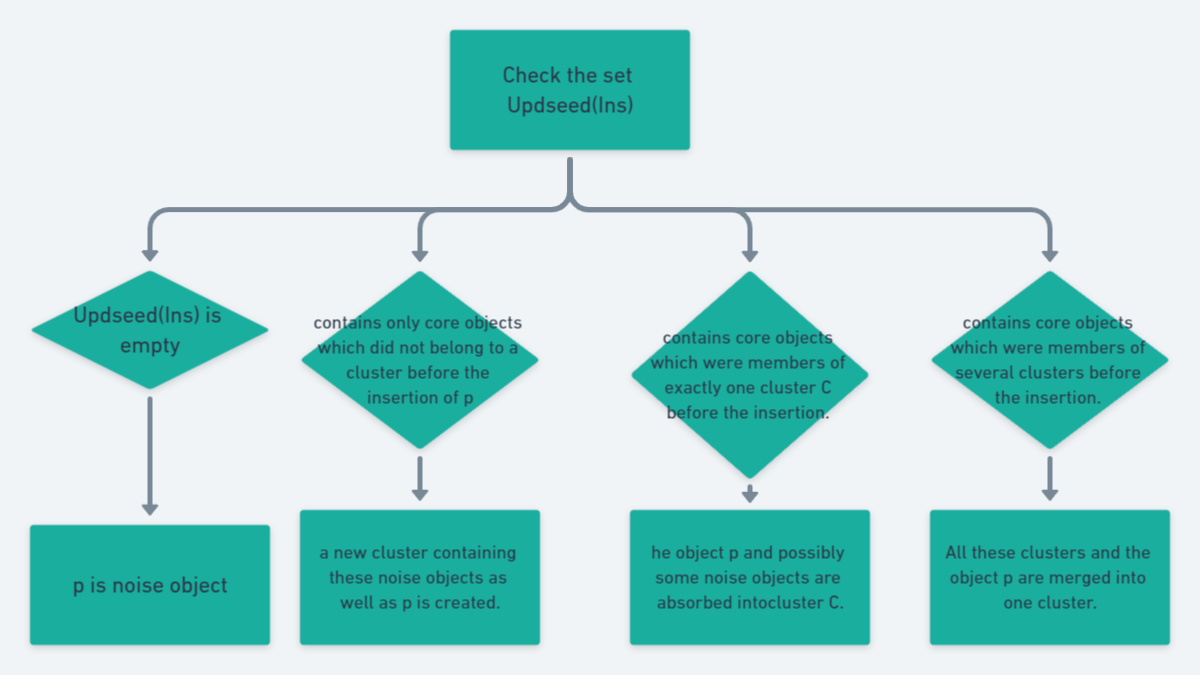
\includegraphics[width = \textwidth]{Flowchart Insertion Cluster Assignment.png}
            \caption{Insertion of point}
            \label{fig:my_label}
        \end{figure}
        
        \item \textbf{Deletion of a point: }
        As opposed to an insertion, when deleting an object p, density-connections may be removed, but no new connections are established. The difficult case for deletion occurs when the cluster C of p is no longer density-connected via (previous) core objects in N\textsubscript{$\epsilon$}(p) after deleting p. In this case, we do not know in general how many objects we have to check before it can be determined whether C has to be split or not. In most cases, however, this set of objects is very small because the split of a cluster is not very frequent and in general a non-split situation will be detected in a small neighborhood of the deleted object p. 
        When deleting an object p from the database D we can distinguish the following cases:
        \\ 
        \begin{enumerate}
            \item \textbf{Removal: } \textit{UpdSeed\textsubscript{Del}} is empty, i.e. there are no core objects in the neighborhood of objects that may have lost their core object property after the deletion of p. Then p is deleted from D and eventually other objects in N\textsubscript{$\epsilon$}(p) change from a former cluster C to noise. If this happens, the cluster C is completely removed because then C cannot have core objects outside of N\textsubscript{$\epsilon$}(p).
            \item \textbf{Reduction: } All objects in \textit{UpdSeed\textsubscript{Del}} are directly density-reachable
            from each other. Then p is deleted from D and some objects in N\textsubscript{$\epsilon$}(p) may become noise.
            \item \textbf{Potential Split: } The objects in \textit{UpdSeed\textsubscript{Del}} are not directly density-reachable from each other. These objects belonged to exactly one cluster C before the deletion of p. Now we have to check whether or not these objects are density-connected by other objects in the former cluster C. Depending on the existence of such density-connections, we can distinguish a split and a non-split situation.
        \end{enumerate}
        
        \begin{figure}[!h]
            \centering
            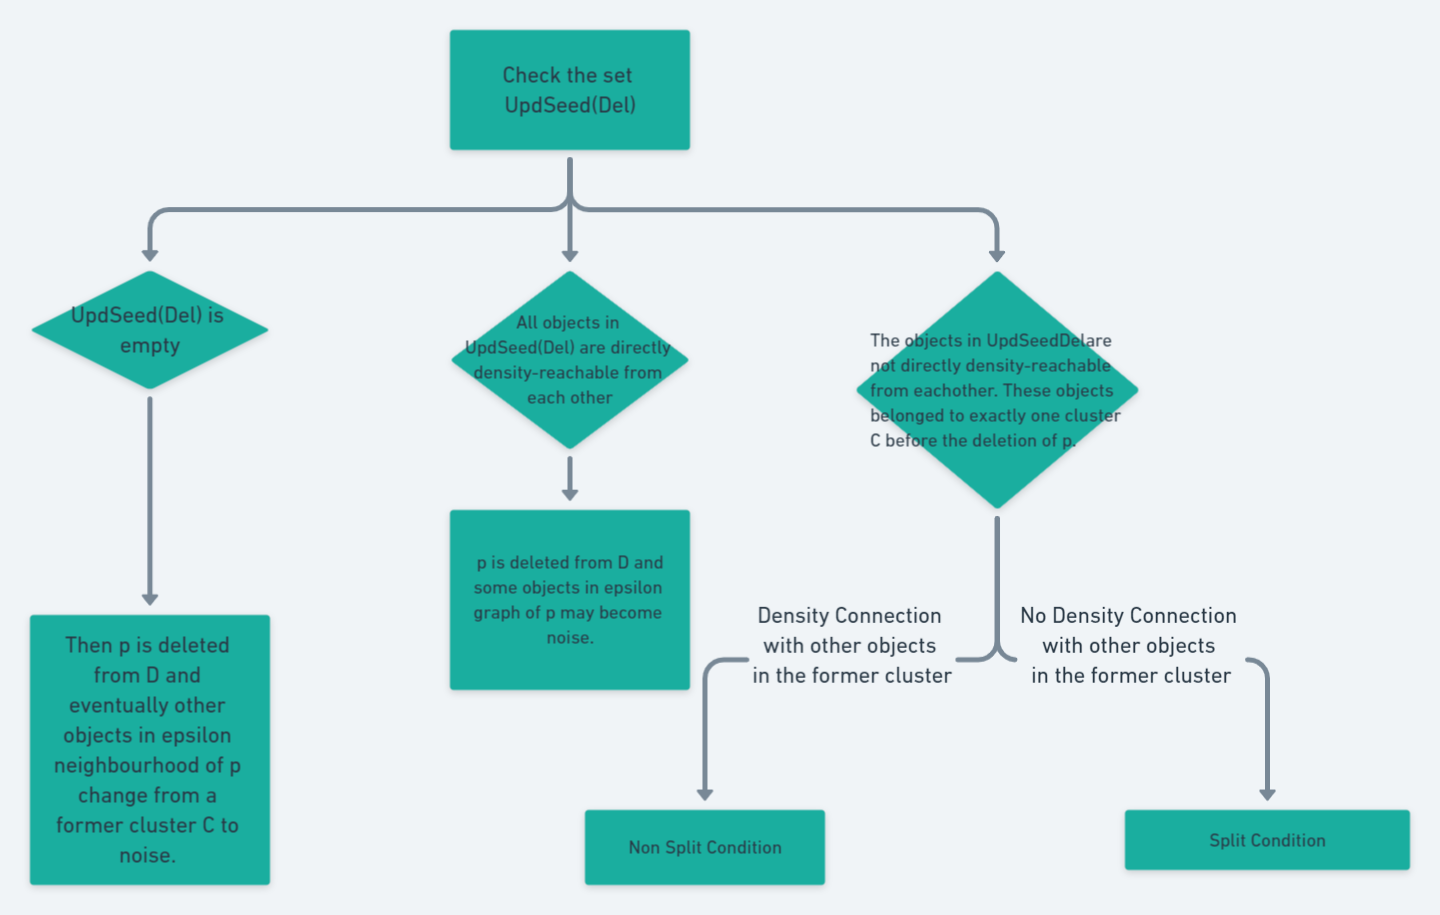
\includegraphics[width = \textwidth]{Flowchart Deletion Cluster Assignment.png}
            \caption{Deletion of point}
            \label{fig:my_label}
        \end{figure}
    \end{itemize}
\end{enumerate}

\section*{Intution of the proposed approach}
Due to the density-based nature of NG-DBSCAN, the insertion or deletion of an object affects the current clustering only in the neighborhood of this object.
\begin{enumerate}
    \item \textbf{Intution for node identification: }To classify each node 'p' as core node, we only need to have \textit{Minpts} number of neighbours within $\epsilon$ distance from 'p'. Hence to gather these \textit{Minpts} neighbours for all points in I, then if in reality there are \textit{Minpts} neighbours for current point in the dataset then we will be able to find such set of points in one or more clusters after some iterations. \newline
    Here we are reducing our computations of finding the $\epsilon$-neighbourhood of whole graph again to only finding it for the points in I. 
    \item \textbf{Intution for finding cluster membership: }We have proved that only for points inside the \textit{UpdSeed\textsubscript{Ins}} and \textit{UpdSeed\textsubscript{Del}} are the nodes for the update related to changing of cluster memberships. \newline 
    Here we are reducing our computations by looking over only certain nodes while performing addition and deletion of points instead of looking over and creating the whole propagation tree and clusters again. 
\end{enumerate}

\section*{Further Work}
In next week we will work on detailed algorithm of Cluster Membership Assignment for insertion and deletion both. We will further compare the percent of time needed to run the whole NG-DBSCAN algorithm with respect to insertion of new coming data objects and determines which approach takes fewer amounts of time and effort.

%%%%%%%%%%%%%%%%%%%%%%%%%%%%%%%%%%%%%%%%%%%%%%%%%%%%%%%%%%%%%%%%%%%%%%%%%%%%%%%

\newpage 
\section* {\centerline{Section 6: Proposed Incremental Algorithm, Iteration 2} \newline}
\addcontentsline{toc}{section}{\large Section 6: Proposed Incremental Algorithm, Iteration 2}

\section*{Introduction}
To increase the novelity of NG-DBSCAN incremental algorithm, we have modified some parts of our incremental algorithm. We have make it batch incremental instead of point by point since less computations are expected to occur in that case. Our incremental version, will read an input file consisting of points to add and delete from the existing dataset D and will read another file consisting of current dataset D and it's clusters and after that it will process all the new points in batch mode. After processing of these updates, we will store the updated dataset D' and clusters C' in the same file which we read earlier since it will be further used while processing updates another time.

\section*{Description of Incremental Version}
Let the dataset of clusters before processing of updates be denoted by D. We have taken the same convention for \textit{Minpts}. A node is core node if it contains more than \textit{Minpts} nodes in it's $\epsilon$-neighbourhood. A node is border node if it has atleast one core node in it's $\epsilon$-neighbourhood. Remaining are noise points. Non-core nodes comprises of border and noise points.

\begin{enumerate}

\item \textbf{Identification of Nodes: }
Here we will approximately identify each node's type (core or non-core) in the updated dataset D' in batch incremental mode. To prevent going over our whole dataset of points, we will seperately maintain border, core, noise points in different sets.

\begin{algorithm}
    \SetAlgoLined
    \KwResult{The updated dataset after addition of points will become labeled with core and non-core points}
    Let all the points to add into the current dataset form a set 'A'. Let all the points having degree less than \textit{Minpts} form a set 'S'\;
    \eIf{A.size * S.size < threshold}{
        For each point in 'S', we will calculate distance with each point in 'A'\;
    }{
        Run the random\_neighbour\_search algorithm for all the points in 'S' over the set 'A'\;
    }
    To identify the type (core or non-core) of newly added points, store them in \textit{\textbf{I}}\;
    Run random\_neighbour\_search algorithm to find the approximate $\epsilon$-neighbourhood of the newly added points to label them\;
    \caption{Node Identification Addition of Points}
\end{algorithm}

\begin{algorithm}
    \SetAlgoLined
    \KwResult{$\epsilon$ Neighbourhood of the given set of points}
    Let S be the set of points for which we have to find $\epsilon$-neighbourhood over set A\;
    \eIf{A is Old Cluster Data}{
        Assign each point u of S with k random points from each cluster C (in old cluster)\;
    }{
        Assign each point u of S with k random points in A\;
    }
    Store these random points in T\;
    For each vertex u in S:
    \While{i < iter}{
        For each vertex v in T, check distance between u and v\;
        \eIf{dis(u,v) <= $\epsilon$}{
            Create an edge between u and v in $\epsilon$ Neighbourhood Graph\;
            Insert neighbours of v in T\;
        }{
            Check for another vertex in T\;
        }
        i++\;
    }
    \caption{Random Neighbour Search Algorithm}
\end{algorithm}
   
\begin{figure}[H]
    \centering
    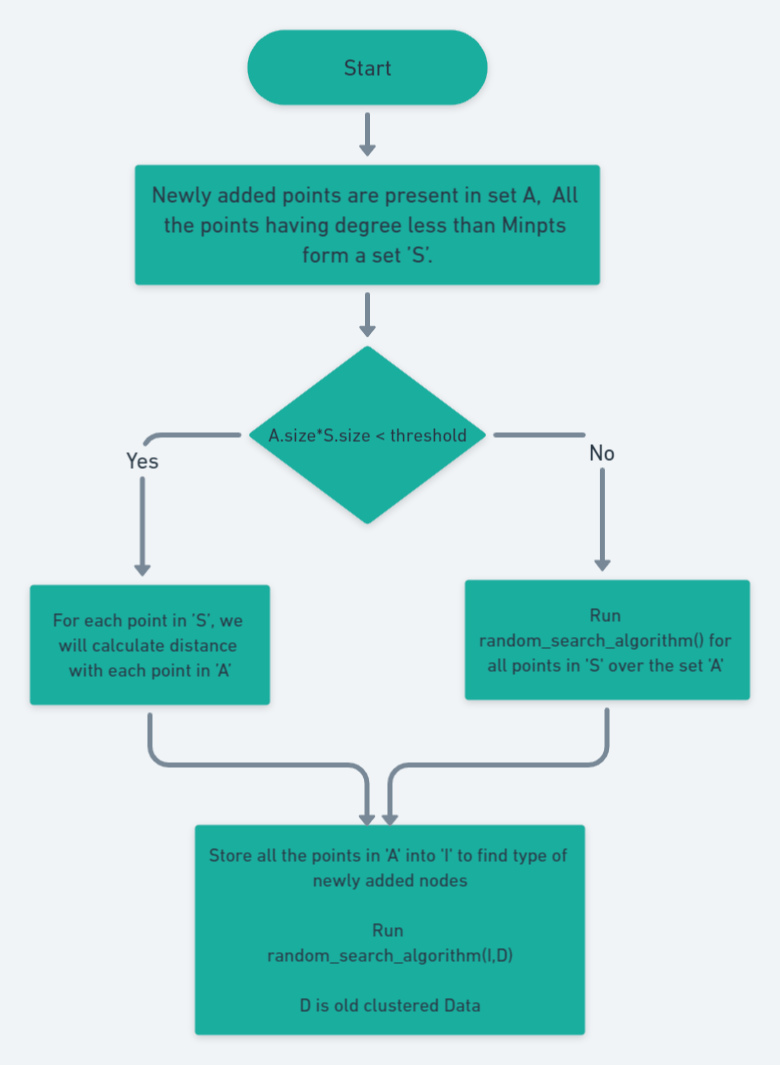
\includegraphics[height = 0.6\textheight, width = \textwidth, keepaspectratio]{Node_identification.png}
   \caption{Identifying Affected Nodes in Addition of Points}
    \label{fig:my_label}
\end{figure}
        
\begin{figure}[H]
    \centering
    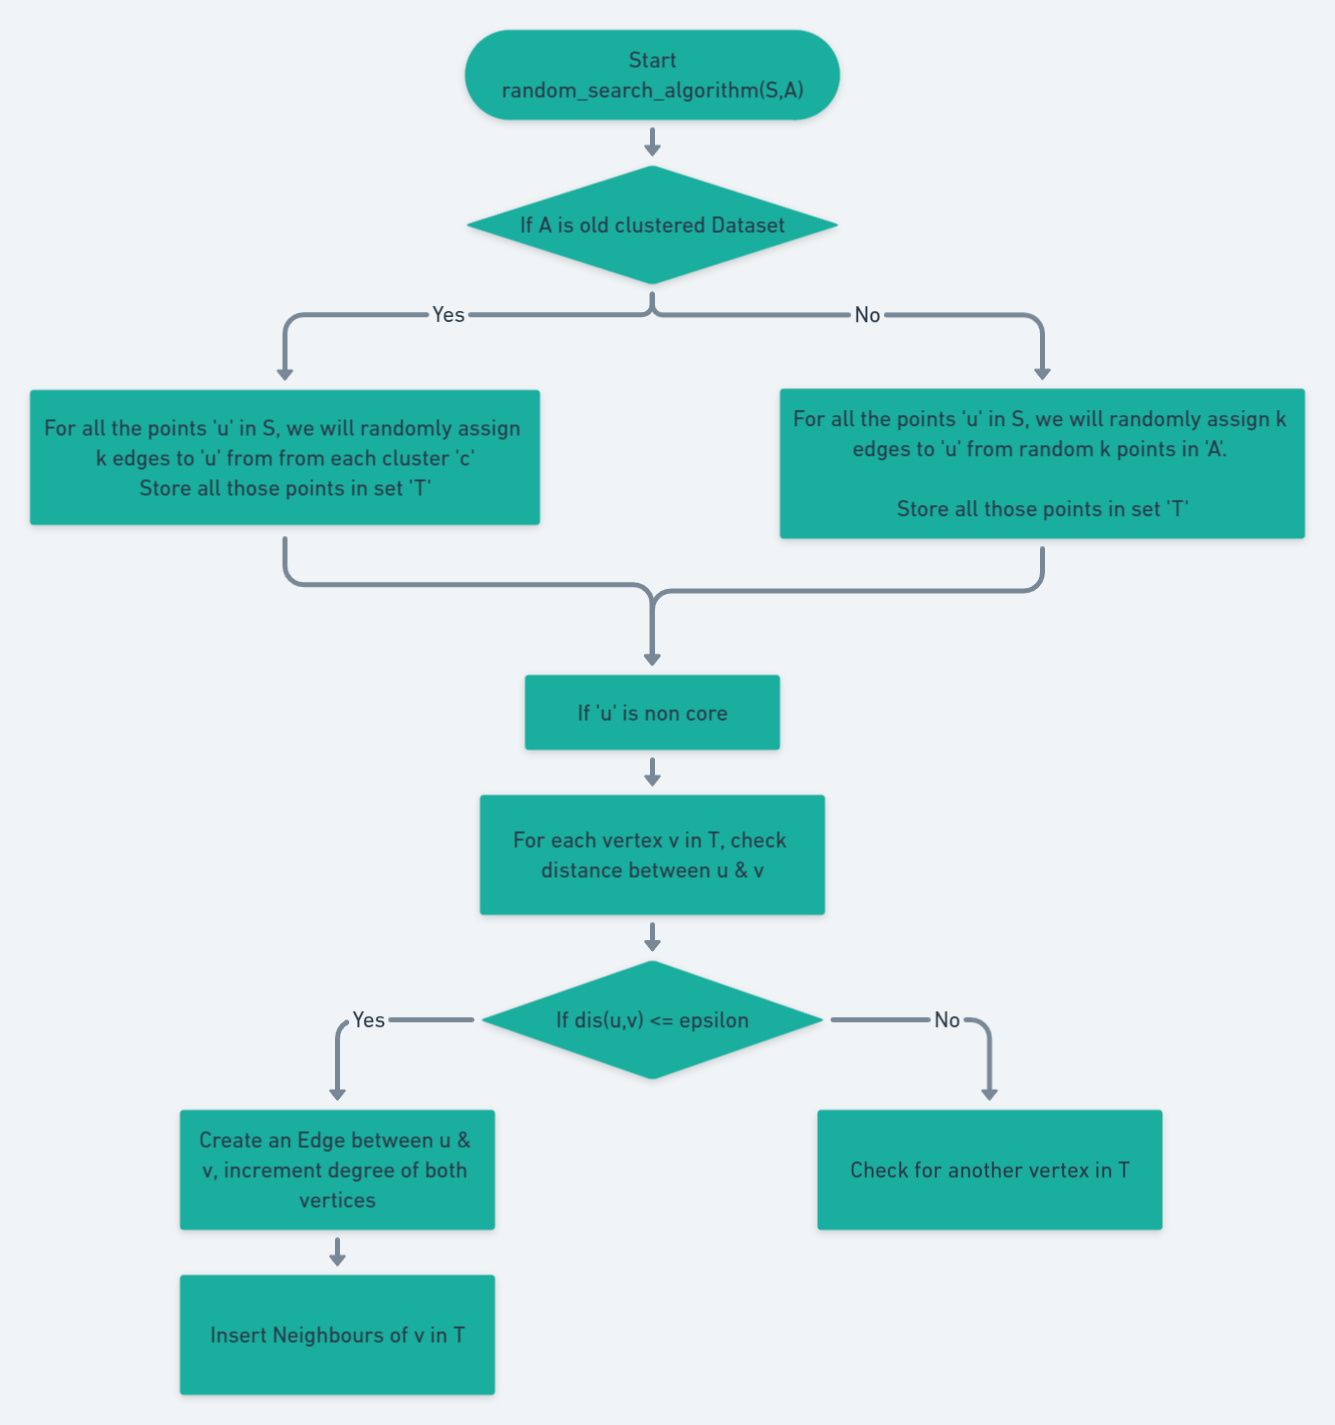
\includegraphics[height = 0.6\textheight, width = \textwidth, keepaspectratio]{random_search_algorithm.png}
    \caption{Random Search Algorithm}
    \label{fig:my_label}
\end{figure}  

\begin{algorithm}
    \SetAlgoLined
    \KwResult{The updated dataset after deletion of points will become labeled with core and non-core points}
    Let all the points to delete from the current dataset, form a set 'D'. Let all the points having degree more than or equal to \textit{Minpts} form a set 'R'\;
    For all the points in 'R', calculate which all points will lose their degree to < Minpts after deleting the points present in 'D'. This can be done by going over the neighbour list of each point in 'R'\;
    Store all these points which will have their final degree < Minpts in 'I'\;
    Run random\_neighbour\_search algorithm for points in I over dataset D so that we could find whether they can become core or not again\;
    \caption{Node Identification Deletion of Points}
\end{algorithm}
\begin{figure}[H]
    \centering
    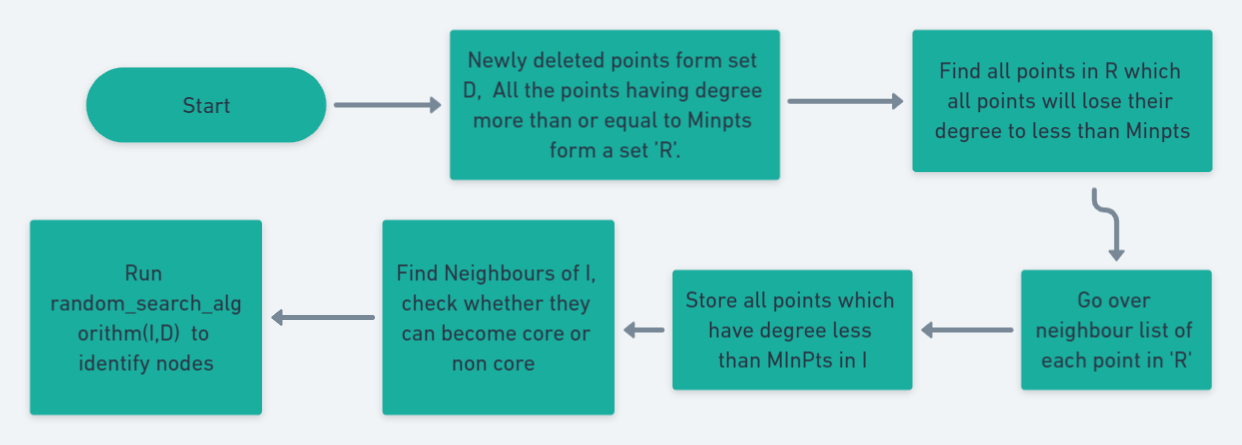
\includegraphics[width = \textwidth]{deletion OF Node.png}
    \caption{Deletion Of Points}
    \label{fig:my_label}
\end{figure}

\item \textbf{Cluster Membership :}
In the cluster membership process, each node will get it's label (core or non-core) in the updated dataset D'.
\begin{algorithm}
    \SetAlgoLined
    \KwResult{The updated dataset after addition of points will be clustered}
    From the identification of nodes section, we can identify which nodes have changed their identity from non-core to core. So, store these points in a set 'Upd\textsubscript{ins}'\;
    After building this set, Depth First Search will run from all points in 'Upd\textsubscript{ins}' and give each point the cluster number to which it belongs\;
    In each DFS, unique and same cluster name is given to all points which are reachable from that point\;
    Each point is visited once only in this process in the updated dataset D'\;
    \caption{Cluster Membership Addition of Points}
\end{algorithm}
\begin{figure}[H]
    \centering
    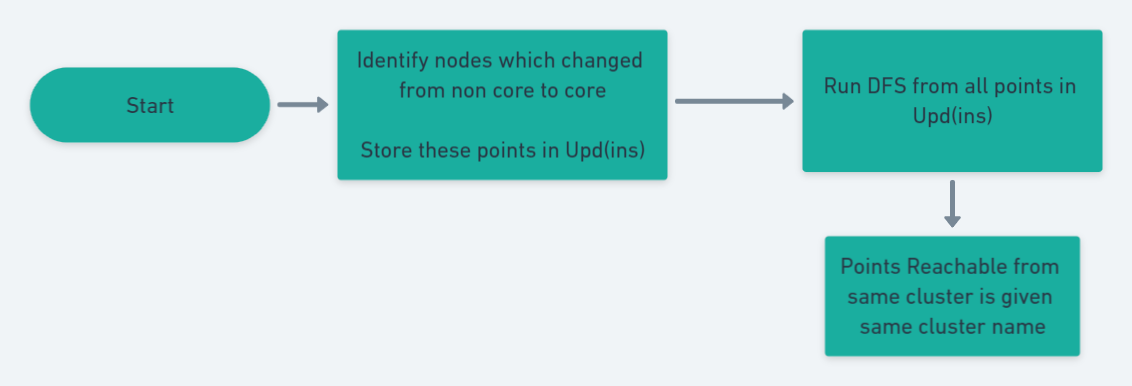
\includegraphics[width = \textwidth]{cluster_membership_addition.png}
    \caption{Addition Of Points}
    \label{fig:my_label}
\end{figure} 
\begin{algorithm}
    \KwResult{The updated dataset after deletion of points will be clustered}
    From the identification of nodes section, we can identify which nodes have changed their identity from core to non-core. So, store these points in a set 'Upd\textsubscript{del}'\;
    After building this set, run Depth First Search from all points in 'Upd\textsubscript{del}' and give each point the cluster number to which it belongs\;
    In each DFS, unique and same cluster name is given to all points which are reachable from that point\;
    Each point is visited once only in this process in the updated dataset D'\;
    \caption{Cluster Membership Deletion of Points}
\end{algorithm}

\begin{figure}[H]
    \centering
    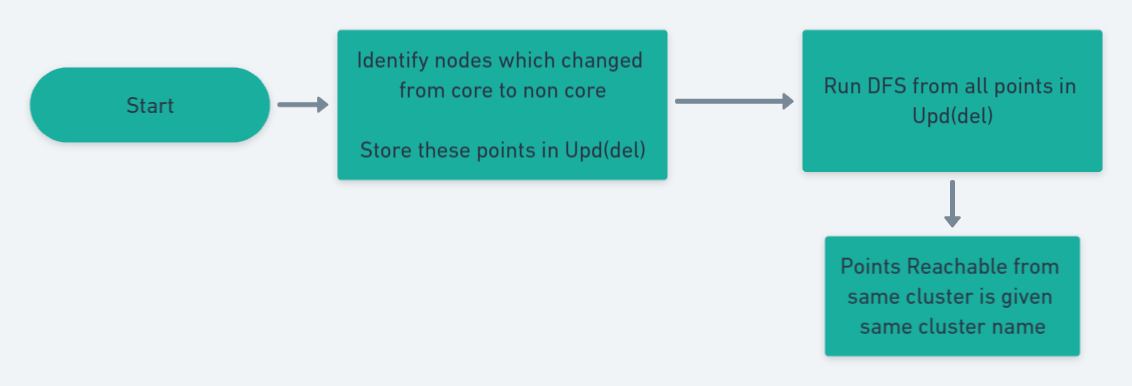
\includegraphics[width = \textwidth]{cluster_membership_deletion.png}
    \caption{Deletion Of Point}
    \label{fig:my_label}
\end{figure}
\end{enumerate}

\section*{Comparison with Static Version}
In the node identification step, we are continuously updating our $\epsilon$-graph , maintaining the degree of each node, maintaining the $\epsilon$-graph where each node will have maximum $M\textsubscript{max}$ number of neighbours which we also did in the phase 1 of the static version of NG-DBSCAN algorithm. In this step of incremental version of the algorithm we are only traversing the newly added points to find $\epsilon$ neighbourhood of the point thus saving us from large time usage. \newline
In the cluster membership step, we are running the Depth First Search which we also did in static version to find all the numbered clusters. \newline 
We didn't use the max selection and pruning step from phase 2 of our static algorithm in the incremental version since they will increase the computational cost by going over the whole dataset for multiple iterations.  

\section*{Complexity of Incremental Version}
\begin{itemize}
    \item \textbf{Node Identification Part: } Time complexity will be linear to the number of points in the updated dataset.
    \vspace{3pt}
    \begin{itemize}
        \item \textbf{Addition: }First step of addition will take $O(n*a)$ where 'n' is the number of non-core points in the dataset D before update and 'a' is the number of points to be added in D. Second step of addition will take $O(a*c)$ where 'c' is the constant number of iterations for which we will search for the neighbours for each point in I. 
        \vspace{3pt}
        \item \textbf{Deletion: }First step of deletion will take $O(m)$ where 'm' is the number of core points in the dataset D before update. Second step of deletion will take $O(m*c)$ where 'c' is the constant number of iterations for which we will search for the neighbours for each point in I. 
    \end{itemize}
    \vspace{4pt}
    \item \textbf{Cluster Membership: }Both addition and deletion steps will take $O(N*Minpts)$ time in worst case where 'N' is the number of points in the updated dataset.
\end{itemize}

\section*{Correctness of Algorithm}
\begin{enumerate}
    \item \textbf{Identification of nodes: }
    \vspace{2pt}
    \begin{itemize}
        \item \textbf{Addition: }For all the points present in dataset D, we will get it's approximate type whether it is core or non-core. Also for all the new added points, we found it's neighbours in each cluster hence we also get an approximation of the cluster to which it will belong along with it's type. Hence each node will have it's approximate type.
        \vspace{2pt}
        \item \textbf{Deletion: }All the points in I will be those which can change from core to non-core. But some of them can still become core by having some connections in the dataset and we found those nodes through random\_neighbour\_search. Hence here also each node will have it's approximate type in the updated dataset.
    \end{itemize}
    \vspace{3pt}
    \item \textbf{Cluster Membership: }Since we are running DFS from all those points which got their type changed, all the reachable nodes from these affected nodes are visited and their cluster numbers are updated. All the other remaining points will have their previous cluster numbers since addition and deletion of points didn't affected them.
\end{enumerate}

\section*{Code Architecture}
\begin{enumerate}
    \item \textbf{Data Structures}
    \begin{enumerate}
        \item \textit{Input Data Representation: } The dataset before updates will be stored in prev\_data.txt and the clusters of that dataset will be stored in clusters.txt. The points to be added or deleted will be stored in queries.txt. Each point to be added will be represented by "A point" and to be deleted by "D point" in queries.txt where 'point' is the node to add or delete.
        \item \textit{Data Generated: } The updated dataset D' will be stored in prev\_data.txt and it's newly identified clustering will be stored in clusters.txt.
    \end{enumerate}
    \vspace{3pt}
    \item \textbf{Class and Methods Overview}
    \begin{itemize}
        \item \textit{Class Node: } This class contains all the information regarding the node.
        \item \textit{Class Parameter:} This class contains all the parameters. \newline Attributes: Minpts, M\textsubscript{max}, threshold, k, iter.
        \item \textit{Class Graph: } This class represents the whole graph.
        Attributes: set of ids of present nodes, total no of nodes, edge lists, coordinates of each node, dimension of dataset. 
        Methods: add\_edge, remove\_edge, insert\_node, delete\_node.
        \item \textit{points\_addition: }This method is used to classify the type of the updated dataset after insertion. \newline
        Input Parameters: Set of points to be added.
        \item \textit{points\_deletion: }This method is used to classify the type of the updated dataset after deletion. \newline
        Input Parameters: Set of points to be deleted.
        \item \textit{random\_neighbour\_search: }This method is used to find for each node 'u' in 'S', it's neighbours in 'A' to classify them.
        Input Parameters: Set 'A', 'S', 'I'.
        \item \textit{cluster\_assignment: }This method is used to classify all the reachable points from each other the same cluster number.
        Input Parameters: cluster number, node, $\epsilon$-graph, set of visited nodes.
    \end{itemize}
\end{enumerate}

\section*{Further Work}
In the upcoming weeks, we will implement the incremental version in C++ and will also try to experimentally evaluate it using different metrics of recall, seperation, compactness. We will also compare the static and incremental version in terms of time, space complexity and using different evaluation metrics which we stated earlier in our report. 

\newpage

\section* {\centerline{Section 7: Experimental Results, Iteration 1} \newline}
\addcontentsline{toc}{section}{\large Section 7: Experimental Results, Iteration 1}

\section*{Introduction}
This week we have implemented our Incremental NG-DBSCAN algorithm. In order to handle the need of Incremental version we have modified static version of NG-DBSCAN. We have generated datasets to test our algorithm and calculate the experimental results. \\ \\ We first run the static version on the dataset D (points present in points.txt) to generate the clusters. After that we read the queries to add and delete data points, then run the incremental algorithm. To compare the results of incremental version with static version we run the static version of changed dataset D$'$. We then compare the metrics and resources used by both versions of the algorithm.

\section*{Code Files}
In our github repository, the folder named "Incremental NG-DBSCAN" contains the incremental version code and the dataset used. Here is the description of the folders and the files:
\begin{enumerate}
    \item \textbf{Dataset\_1: }This folder contains the points.txt, queries.txt and the experimental result images for our first dataset.
    \item \textbf{Dataset\_2: }This folder contains the points.txt, queries.txt and the experimental result images for our second dataset.
    \item \textbf{Files: }This folder contains all the files generated by the incremental and static version of NG-DBSCAN used as a database.
        \begin{itemize}
            \item \textit{queries.txt}
            \item \textit{points.txt}
            \item \textit{clusters\_save.txt}
            \item \textit{clusters\_save1.txt}
            \item \textit{points\_save.txt}
            \item \textit{points\_save1.txt}
            \item \textit{epsilon\_graph\_save.txt}
            \item \textit{epsilon\_graph\_save1.txt}
        \end{itemize}
    \item \textbf{Static: }This folder contains the static version code with minor modifications done to compare static NG-DBSCAN results with incremental NG-DBSCAN results.
    \item \textbf{static\_ngdbscan.cpp: }It contains the main c++ code to run the static NG-DBSCAN code. 
    \item \textbf{incr\_ngdbscan.cpp: }It contains the whole c++ incremental NG-DBSCAN code.
    \item \textbf{incr\_classes.h: }It contains the classes used while implementing incremental NG-DBSCAN code.
    \item \textbf{metrics\_calculate: }It contains the functions of compactness and seperation to compare the accuracy of static and incremental version.
    \item \textbf{metrics\_main: }It contains the main code to calculate accuracy of static and incremental NG-DBSCAN code.
    \item \textbf{clusters\_generator.py: }It is used to plot the clusters by using the files \textit{points\_save.py} and \textit{clusters\_save.py}.
\end{enumerate}

\section*{Datasets}
Till now we have only evaluated and compared our incremental version with static version on 2-dimensional datasets. We have only used 2 synthetically generated datasets till now. \textit{points.txt} contains the points of the dataset. \textit{queries.txt} contains points to add and delete.
\begin{enumerate}
    \item \textbf{Dataset\_1: }Contains \textit{points.txt}, \textit{queries.txt} and \textit{dataset\_1.py} files. \textit{dataset\_1.py} contains code to generate this dataset.
    \item \textbf{Dataset\_2: }Contains \textit{points.txt}, \textit{queries.txt} and \textit{dataset\_2.py} files. \textit{dataset\_2.py} contains code to generate this dataset.
\end{enumerate}
We have used \textit{clusters\_save.txt}, \textit{points\_save.txt} and \textit{epsilon\_graph\_save.txt} to save the dataset after running \textit{points.txt} over the static version of NG-DBSCAN. Then we have used \textit{queries.txt} over this saved dataset in both static and incremental version to generate changed dataset having names \textit{clusters\_save1.txt}, \textit{points\_save1.txt} and \textit{epsilon\_graph\_save1.txt} which are further used in calculating metrics and cluster plots for the dataset.

\section*{Comparison with static version}
For static, we have formed new dataset D' by adding and deleting the corresponding data points. Then we run the static version of the algorithm on the dataset D'.
\begin{enumerate}
    \item \textbf{Time and Memory: }\\
        We have calculated time used by our program (excluding read and writing to text files). \\
        \begin{itemize}
            \item \textit{\textbf{Dataset 1}} 
                \begin{figure} [H]
                    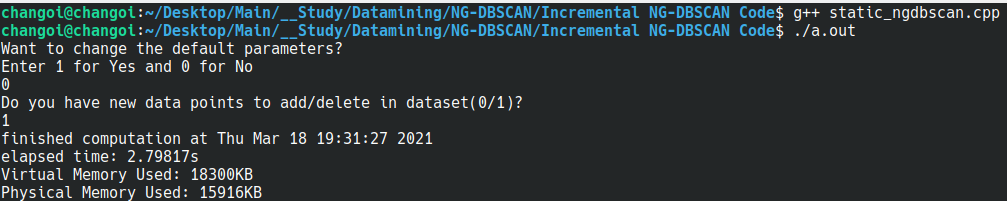
\includegraphics[width=\textwidth]{dataset_1_new_static_run.png}
                    \caption{Static on Dataset 1} 
                \end{figure}
                    
                \begin{figure} [H]
                    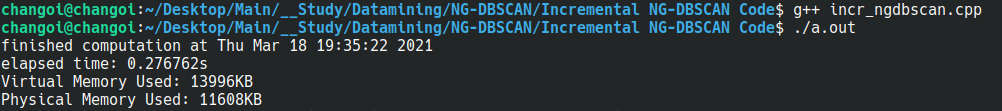
\includegraphics[width=\textwidth]{dataset_1_incr_run.png}
                    \caption{Incremental on Dataset 1} 
                \end{figure}
                
            \item \textit{\textbf{Dataset 2}}
                \begin{figure} [H]
                    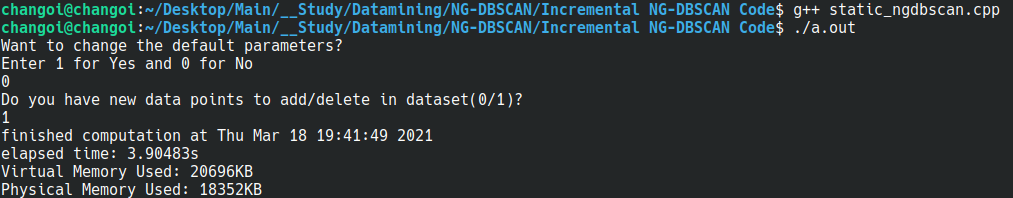
\includegraphics[width=\textwidth]{dataset_2_new_static_run.png}
                    \caption{Static on Dataset 2}
                \end{figure}
                    
                \begin{figure} [H]
                    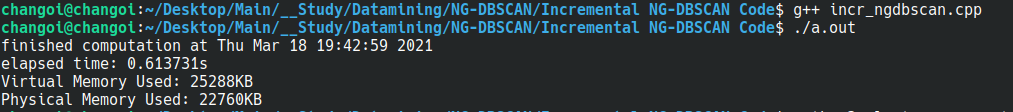
\includegraphics[width=\textwidth]{dataset_2_incr_run.png}
                    \caption{Incremental on Dataset 2}
                \end{figure}
        \end{itemize}
        \textbf{Explanation for above results: } Incremental algorithm is 7 to 10 times better compared to static algorithm. Extra time saved is due to use of old clustered data and generating two sets \textit{upd\_ins}(it contains point which have changed their property from non core to core) and \textit{upd\_del}(it contains point which have changed their property from core to non core) to find new clusters instead of whole datasets.
        \vspace{2pt}
    \item \textbf{Accuracy: }
        We have used metrics \textbf{Compactness} and \textbf{Separation} for calculating accuracy.
        \begin{figure} [H]
            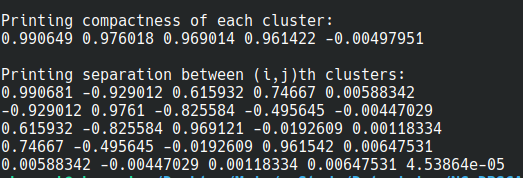
\includegraphics[]{dataset_1_old_static_metric.png}
            \caption{Static on Dataset 1} 
        \end{figure}
        
        \begin{figure} [H]
            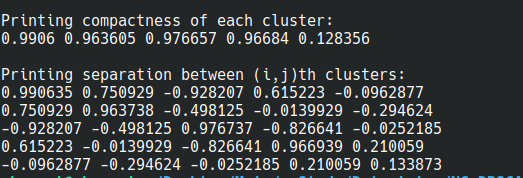
\includegraphics[]{dataset_1_new_static_metric.png}
            \caption{Static on Dataset 1, After addition/deletion of Points} 
        \end{figure}
                    
        \begin{figure} [H]
            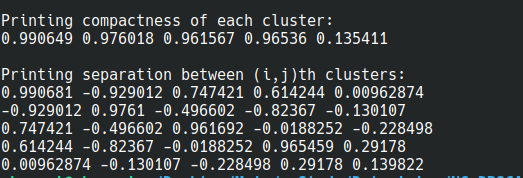
\includegraphics[]{dataset_1_incr_metric.png}
            \caption{Incremental on Dataset 1} 
        \end{figure}
                    
        \begin{figure} [H]
            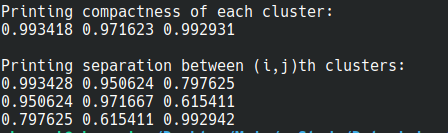
\includegraphics[]{dataset_2_old_static_metric.png}
            \caption{Static on Dataset 2} 
        \end{figure}
                    
        \begin{figure} [H]
            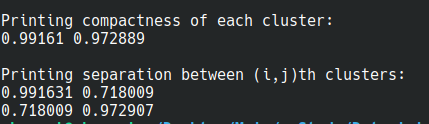
\includegraphics[]{dataset_2_new_static_metric.png}
            \caption{Static on Dataset 2, After addition/deletion of Points} 
        \end{figure}
        
        \begin{figure} [H]
            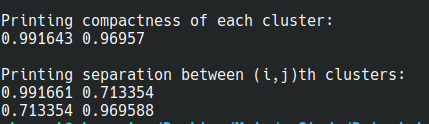
\includegraphics[]{dataset_2_incr_metric.png}
            \caption{Incremental on Dataset 2} 
        \end{figure}
                    
        \textbf{Explanation for above results: } Compactness is similar in both incremental and static version. But in seperation, for some clusters it is not less in incremental version, may be due to the random point assignment from each cluster to the set of added and deleted points. 
        \vspace{2pt}
            
        \item \textbf{Comparison with Graphs: }We have plotted the clusters in 2-dimensional for both incremental and static version and compared them.
        \vspace{-20mm}
            \begin{figure} [H]
                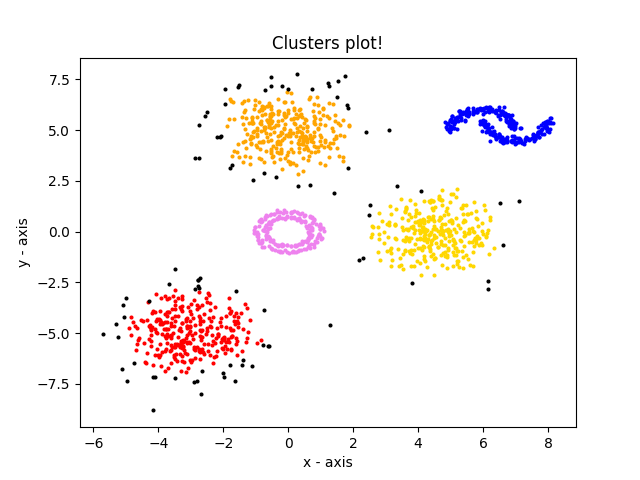
\includegraphics[scale = 0.72]{dataset_1_old_static.png}
                \caption{Static on Dataset 1} 
            \end{figure}
                    
            \begin{figure} [H]
                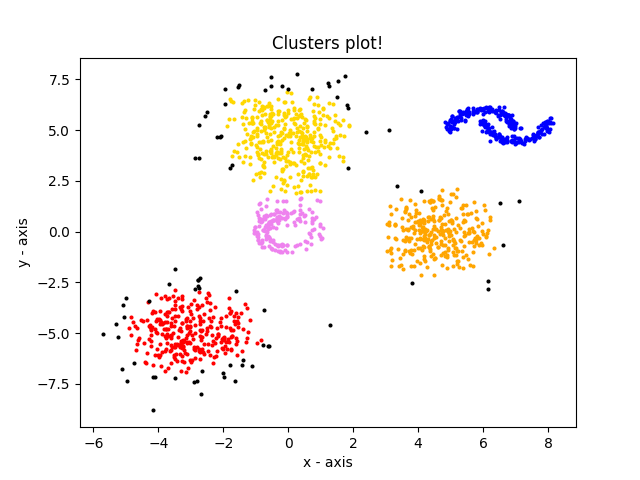
\includegraphics[scale = 0.72]{dataset_1_new_static.png}
                \caption{Static on Dataset 1, After addition/deletion of Points} 
            \end{figure}
            
            \begin{figure} [H]
                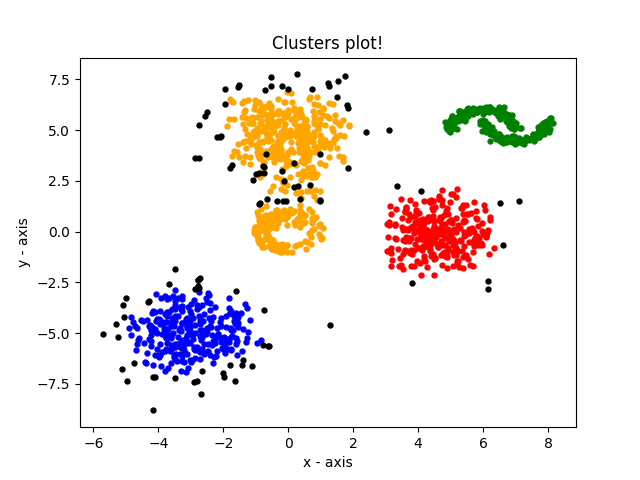
\includegraphics[scale = 0.72]{dataset_1_incr.png}
                \caption{Incremental on Dataset 1} 
            \end{figure}
                    
            \begin{figure} [H]
                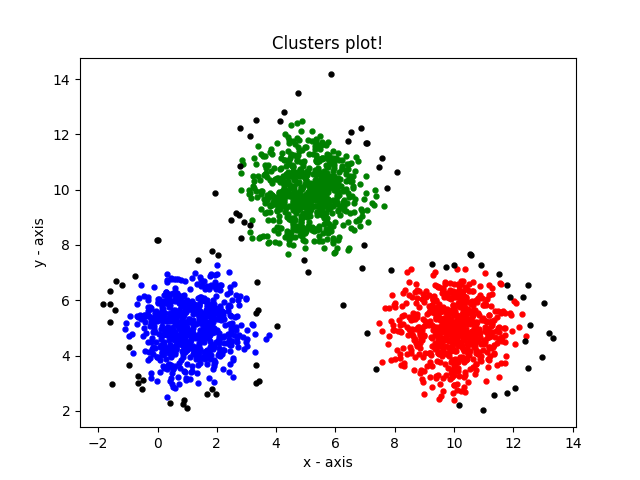
\includegraphics[scale = 0.72]{dataset_2_old_static.png}
                \caption{Static on Dataset 2} 
            \end{figure}
            
            \begin{figure} [H]
                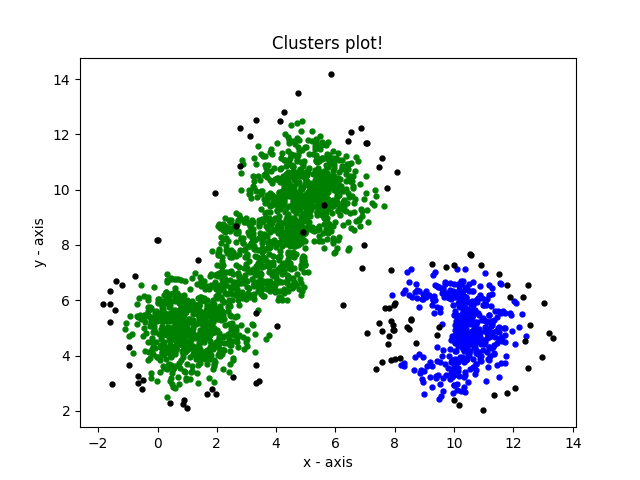
\includegraphics[scale = 0.72]{dataset_2_new_static.png}
                \caption{Static on Dataset 2, After addition/deletion of Points} 
            \end{figure}
            
            \begin{figure} [H]
                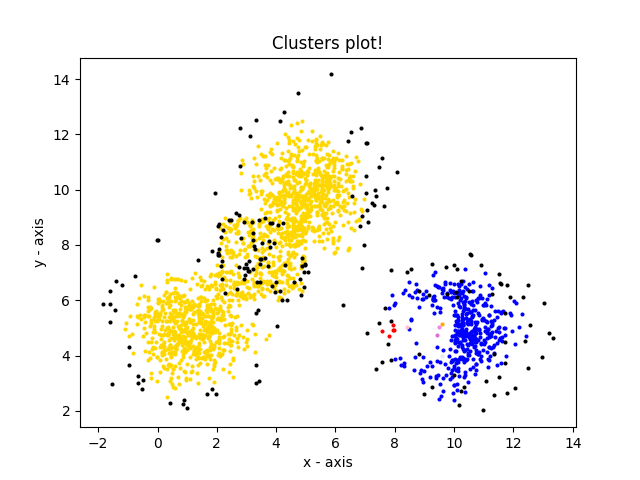
\includegraphics[scale = 0.72]{dataset_2_incr.png}
                \caption{Incremental on Dataset 2} 
            \end{figure}
                
            \textbf{Explanation for the results: } Incremental algorithm has lesser accuracy and cluster quality compared to static algorithm, because we are randomly selecting points and pruning the dataset to select only handful of points to run the algorithm instead of running it on whole dataset.
\end{enumerate}

\section*{Further Work}
In the further week, we will implement the incremental version with n-dimensional dataset and with more number of add and delete queries and more number of points in the dataset. We will also evaluate our algorithm with recall metric to calculate accuracy. We will also try to tune our parameters to make our incremental algorithm more accurate.

\end{document}